%===============================================================================
% LaTeX sjabloon voor de bachelorproef toegepaste informatica aan HOGENT
% Meer info op https://github.com/HoGentTIN/bachproef-latex-sjabloon
%===============================================================================
\documentclass{bachproef-tin}
\usepackage{hogent-thesis-titlepage} % Titelpagina conform aan HOGENT huisstijl

\usepackage[nonumberlist]{glossaries}
\renewcommand{\glossarysection}[2][]{} % Fix voor glossary met HoGent Theme
\makeglossaries
%run generate.sh en run hier
\newglossaryentry{datacompressie}
{
	name={datacompressie},
	description={Datacompressie bestaat uit het digitaal opslaan van een bestand met zo weinig mogelijk bits. Enkele belangrijke factoren voor het bepalen van de juiste datacompressie zijn gewenste kwaliteit, bestandsgrootte en snelheid}
}

\newglossaryentry{bit}
{
	name={bit},
	description={Zoals de naam bit, kort voor binary digit, suggereert kan een bit beschouwd worden als een binair signaal. Een bit wordt beschouwd als de kleinste data eenheid voor dataopslag. Meer informatie rond bestandsgrootte en dataopslag worden besproken in hoofdstuk \ref{ch:literatuurstudie}, deel \ref{sec:bestandsgrootte-dataopslag}},
	plural={bits}
}

\newglossaryentry{dna-compressie}
{
	name={DNA compressie},
	description={Het menselijke DNA kan digitaal voorgesteld worden door een lange lijst van 5 verschillende karakters, gekend als basen. Deze digitale voorstelling bestaat uit meer dan 3 miljard van deze basen (\cite{dodanaugent2011}). DNA compressie bestaat er uit deze reeks van basen zo efficiënt mogelijk op te slaan zodanig dat performante bewerkingen mogelijk zijn met een zo klein mogelijke bestandsgrootte}
}

\newglossaryentry{afbeeldingscompressie}
{
	name={afbeeldingscompressie},
	description={Afbeeldingscomspressie bestaat er uit een afbeelding in zo weinig mogelijk aantal bits op te slaan terwijl een accapteerbare kwaliteit behouden blijft. Dit kan zowel via lossless als lossy algoritmes. Afbeeldingscompressie wordt uitgebreid besproken in hoofdstuk \ref{ch:afbeeldingscompressie}}
}

\newglossaryentry{videocompressie}
{
	name={videocompressie},
	description={Videocompressie bestaat er uit een videobstand in zo weinig mogelijk aantal bits op te slaan terwijl een accapteerbare kwaliteit behouden blijft. Dit kan zowel via lossless als lossy algoritmes. videcompressie wordt uitgebreid besproken in hoofdstuk \ref{ch:videocompressie}}
}

\newglossaryentry{codec}
{
	name={codec},
	description={Binnen datacompressie betekent codec de gebruikte techniek om een bestand te comprimeren. De codec is dus is de technologie verantwoordelijk voor het encoden en decoden van een bestand volgens een bapaald compressiealgoritme. BV; H.265},
	plural={codecs}
}

\newglossaryentry{afbeeldingsformaat}
{
	name={afbeeldingsformaat},
	description={Een afbeeldingsformaat bevat alle gegevens voor het digitaal opslaan van een afbeelding. De vier gekendste categoriën van afbeeldingsformaten zijn: raster, vector, compound en stereo formaten},
	plural={afbeeldingsformaten}
}

\newglossaryentry{container}
{
	name={container},
	description={Binnen datacompressie kan een container vrijwel letterlijk vertaald worden. Het is een verpakking voor alle data die men opslaat alsook de instructies voor het openen van die data. onder andere de codec plaatst data in deze container. Wanneer er gesproken wordt over bestandsextensies wordt vaak de container bedoeld. Bv; MP4 }
}

\newglossaryentry{jpeg}
{
	name={JPEG},
	description={Ook gekend als JPG. JPEG is een afkorting voor Joint Photographic Experts Group. JPEG is een bestandsformaat voor het opslaan van digitale afbeeldingen via lossy compressie. Afbeeldingscompressie en JPEG worden uitgebreid besproken in hoofdstuk \ref{ch:afbeeldingscompressie}}
}

\newglossaryentry{jpeg2000}
{
	name={JPEG2000},
	description={Ook gekend als JPEG2K. JPEG2000 is een bestandsformaat voor het opslaan van digitale afbeeldingen gemaakt als opvolger van JPEG. Net zoals JPEG maakt het gebruik van lossy compressie. Afbeeldingscompressie en JPEG2000 worden uitgebreid besproken in hoofdstuk \ref{ch:afbeeldingscompressie}}
}

\newglossaryentry{png}
{
	name={PNG},
	description={PNG is een afkorting voor Portable Network Graphics. PNG is een bestandsformaat voor het opslaan van digitale afbeeldingen. PNG maakt gebruik van lossless compressie. Afbeeldingscompressie en PNG worden uitgebreid besproken in hoofdstuk \ref{ch:afbeeldingscompressie}}
}

\newglossaryentry{h264-avc}
{
	name={H.264-AVC},
	description={H.264-AVC is één van de gekenste videocodecs die grootschalig gebruikt wordt. AVC is een afkorting van Advanced Video Coding. Videocompresssie en H.264-AVC worden uitgebreid besproken in hoofdstuk \ref{ch:videocompressie}}
}
% TODO: veruidelijken als deel geschreven is.

\newglossaryentry{h264-svc}
{
	name={H.264-SVC},
	description={H.264-SVC is een videocodec ontwikkelt als extensie van H264-AVC. SVC is een afkorting voor Scalable Video Coding. De nadruk bij deze extensie ligt zoals de naam sugereert op schaalbaarheid. Videocompresssie en H.264-SVC worden uitgebreid besproken in hoofdstuk \ref{ch:videocompressie}}
}
% TODO: veruidelijken als deel geschreven is.

\newglossaryentry{h265}
{
	name={H.265},
	description={H.265 is een videocodec ontwikkelt als opvolger van H.264. Videocompresssie en H.265 worden uitgebreid besproken in hoofdstuk \ref{ch:videocompressie}}
}
% TODO: veruidelijken als deel geschreven is.

\newglossaryentry{av1}
{
	name={AV1},
	description={AV1 is een videocodec ontwikkelt als open standaard. AV1 is een afkorting voor AOMedia Video. AV1 is vooral interessant omdat het royalty free is en dus geen licentiekosten heeft. Videocompresssie en AV1 worden uitgebreid besproken in hoofdstuk \ref{ch:videocompressie}}
}
% TODO: veruidelijken als deel geschreven is.

\newglossaryentry{open-source}
{
	name={open source},
	description={Als een programmeer project open source is wilt dit zeggen dat de broncode raadpleegbaar is en aanpasbaar is door iedereen. Dit wil echter niet gegarandeerd zeggen dat het software programma gratis is in gebruik.}
}

\newglossaryentry{lossless}
{
	name={lossless},
	description={Binnen datacompressie slaat lossless compressie op het comprimeren van een bestand zonder kwaliteitsverlies. In het geval van video's en afbeeldingen wilt dit zeggen dat een bestand gecomprimeerd met een lossless algoritme visueel dezelfde kwaliteit moet hebben}
}

\newglossaryentry{lossy}
{
	name={lossy},
	description={Binnen datacompressie slaat lossy compressie op het comprimeren van een bestand met mogelijks kwaliteitsverlies voor het besparen van data. In het geval van video's en afbeeldingen wilt dit zeggen dat een bestand gecomprimeerd met een lossy algoritme een significante hoeveelheid aan data en kwaliteit kan verliezen in vergelijking met het originele bestand}
}

\newglossaryentry{afbeeldingsevaluatietool}
{
	name={afbeeldingsevaluatietool},
	description={Een software applicatie gemaakt voor het voeren van een objectief of subjectief onderzoek naar afbeeldingskwaliteit. De mogelijke soorten tools worden verder besproken in hoofdstuk \ref{ch:kwaliteit}. Een subjectieve afbeeldingsevaluatietool werd gebouwd voor deze paper en wordt verder besproken in hoofdstuk \ref{ch:onderzoek}}
}

\newglossaryentry{binaire-voorstelling-bestandsgrootte}
{
	name={Binaire voorstelling},
	description={todo}
}
% TODO

\newglossaryentry{si-voorstelling-bestandsgrootte}
{
	name={SI voorstelling},
	description={todo}
}
% TODO

\newglossaryentry{ieee}
{
	name={IEEE},
	description={todo}
}
% TODO

\newglossaryentry{clustergrootte}
{
	name={clustergrootte},
	description={todo}
}
% TODO

\newglossaryentry{cluster}
{
	name={cluster},
	description={todo},
	plural={clusters}
}
% TODO

\newglossaryentry{byte}
{
	name={byte},
	description={todo},
	plural={bytes}
}
% TODO

\newglossaryentry{leestijd}
{
	name={leestijd},
	description={todo},
	plural={leestijden}
}
% TODO

\newglossaryentry{bandbreedte}
{
	name={bandbreedte},
	description={todo}
}
% TODO

\newglossaryentry{prefix-code}
{
	name={prefix code},
	description={todo},
	plural={prefix codes}
}
% TODO

\newglossaryentry{huffman-coding}
{
	name={Huffman coding},
	description={todo}
}
% TODO

\newglossaryentry{frequency-based}
{
	name={frequency based},
	description={todo}
}
% TODO

\newglossaryentry{compressie-algoritme}
{
	name={compressie-algoritme},
	description={todo},
	plural={compressie-algoritmen}
}
% TODO

\newglossaryentry{lookup-table}
{
	name={lookup table},
	description={todo}
}
% TODO

\newglossaryentry{dictionary-coding}
{
	name={dictionary coding},
	description={todo}
}
% TODO

\newglossaryentry{prefix-coding}
{
	name={prefix coding},
	description={todo}
}
% TODO

\newglossaryentry{use-case}
{
	name={use case},
	description={todo},
	plural={use cases}
}
% TODO

\newglossaryentry{rle-long}
{
	name={run length encoding},
	description={todo}
}
% TODO

\newglossaryentry{rle-short}
{
	name={RLE},
	description={Kort voor \gls{rle-long}}
}

\newglossaryentry{ascii}
{
	name={ASCII},
	description={todo}
}
% TODO

\newglossaryentry{encoding}
{
	name={encoding},
	description={todo}
}
% TODO

\newglossaryentry{decoding}
{
	name={decoding},
	description={todo}
}
% TODO

\newglossaryentry{meta-data}
{
	name={meta data},
	description={todo}
}

\newglossaryentry{webp}
{
	name={WEBP},
	description={todo}
}

\newglossaryentry{heic}
{
	name={HEIC},
	description={todo}
}

\newglossaryentry{ps}
{
	name={Adobe Photoshop},
	description={todo}
}

\newglossaryentry{css}
{
	name={CSS},
	description={todo}
}

\newglossaryentry{minifyen}
{
	name={minifyen},
	description={todo}
}

\newglossaryentry{render}
{
	name={render},
	description={todo}
}

\newglossaryentry{raw}
{
	name={RAW},
	description={todo}
}

\newglossaryentry{compressietool}
{
	name={datacompressietool},
	description={todo}
}

\newglossaryentry{github}
{
	name={GitHub},
	description={todo}
}

\newglossaryentry{hosting}
{
	name={hosting},
	description={todo}
}
% TODO

\newglossaryentry{php}
{
	name={PHP},
	description={todo}
}
% TODO

\newglossaryentry{sql}
{
	name={SQL},
	description={todo}
}
% TODO

\newglossaryentry{xampp}
{
	name={XAMPP},
	description={todo}
}

\newglossaryentry{jquery}
{
	name={JQuery},
	description={todo}
}

\newglossaryentry{drift}
{
	name={Drift},
	description={todo}
}

\newglossaryentry{bootstrap}
{
	name={Bootstrap},
	description={todo}
}
% TODO

\newglossaryentry{js}
{
	name={JavaScript},
	description={todo}
}
% 

\newglossaryentry{yt}
{
	name={YouTube},
	description={todo}
}
% TODO

\newglossaryentry{plug-in}
{
	name={plug-in},
	description={todo},
	plural={plug-ins}
}
% TODO

%%---------- Documenteigenschappen ---------------------------------------------
% De titel van het rapport/bachelorproef
\title{Je kijkt er naar, maar ziet het niet: datacompressie	principes - JPEG en PNG - H.264/AVC en H.264/SVC}

% Je eigen naam
\author{Bontinck Lennert}

% De naam van je promotor (lector van de opleiding)
\promotor{Wim De Bruyn}

% De naam van je co-promotor. Als je promotor ook je opdrachtgever is en je
% dus ook inhoudelijk begeleidt (en enkel dan!), mag je dit leeg laten.
\copromotor{Tom Paridaens}

% Indien je bachelorproef in opdracht van/in samenwerking met een bedrijf of
% externe organisatie geschreven is, geef je hier de naam. Zoniet laat je dit
% zoals het is.
\instelling{---}

% Academiejaar
\academiejaar{2018-2019}

% Examenperiode
%  - 1e semester = 1e examenperiode => 1
%  - 2e semester = 2e examenperiode => 2
%  - tweede zit  = 3e examenperiode => 3
\examenperiode{2}

%===============================================================================
% Inhoud document
%===============================================================================

\begin{document}

%---------- Taalselectie -------------------------------------------------------
% Als je je bachelorproef in het Engels schrijft, haal dan onderstaande regel
% uit commentaar. Let op: de tekst op de voorkaft blijft in het Nederlands, en
% dat is ook de bedoeling!

%\selectlanguage{english}

%---------- Titelblad ----------------------------------------------------------
\inserttitlepage

%---------- Samenvatting, voorwoord --------------------------------------------
\usechapterimagefalse
%%=============================================================================
%% Voorwoord
%%=============================================================================

\chapter*{\IfLanguageName{dutch}{Woord vooraf}{Preface}}
\label{ch:voorwoord}

%% TODO:
%% Het voorwoord is het enige deel van de bachelorproef waar je vanuit je
%% eigen standpunt (``ik-vorm'') mag schrijven. Je kan hier bv. motiveren
%% waarom jij het onderwerp wil bespreken.
%% Vergeet ook niet te bedanken wie je geholpen/gesteund/... heeft


%%=============================================================================
%% Samenvatting
%%=============================================================================

% TODO: De "abstract" of samenvatting is een kernachtige (~ 1 blz. voor een
% thesis) synthese van het document.
%
% Deze aspecten moeten zeker aan bod komen:
% - Context: waarom is dit werk belangrijk?
% - Nood: waarom moest dit onderzocht worden?
% - Taak: wat heb je precies gedaan?
% - Object: wat staat in dit document geschreven?
% - Resultaat: wat was het resultaat?
% - Conclusie: wat is/zijn de belangrijkste conclusie(s)?
% - Perspectief: blijven er nog vragen open die in de toekomst nog kunnen
%    onderzocht worden? Wat is een mogelijk vervolg voor jouw onderzoek?
%
% LET OP! Een samenvatting is GEEN voorwoord!

%%---------- Nederlandse samenvatting -----------------------------------------
%
% TODO: Als je je bachelorproef in het Engels schrijft, moet je eerst een
% Nederlandse samenvatting invoegen. Haal daarvoor onderstaande code uit
% commentaar.
% Wie zijn bachelorproef in het Nederlands schrijft, kan dit negeren, de inhoud
% wordt niet in het document ingevoegd.

\IfLanguageName{english}{%
\selectlanguage{dutch}
\chapter*{Samenvatting}
\lipsum[1-4]
\selectlanguage{english}
}{}

%%---------- Samenvatting -----------------------------------------------------
% De samenvatting in de hoofdtaal van het document

\chapter*{\IfLanguageName{dutch}{Samenvatting}{Abstract}}

\lipsum[1-4]


%---------- Inhoudstafel -------------------------------------------------------
\pagestyle{empty} % Geen hoofding
\tableofcontents  % Voeg de inhoudstafel toe
\cleardoublepage  % Zorg dat volgende hoofstuk op een oneven pagina begint
\pagestyle{fancy} % Zet hoofding opnieuw aan

%---------- Kern ---------------------------------------------------------------

% De eerste hoofdstukken van een bachelorproef zijn meestal een inleiding op
% het onderwerp, literatuurstudie en verantwoording methodologie.
% Aarzel niet om een meer beschrijvende titel aan deze hoofstukken te geven of
% om bijvoorbeeld de inleiding en/of stand van zaken over meerdere hoofdstukken
% te verspreiden!

%%=============================================================================
%% Inleiding
%%=============================================================================

\chapter{Inleiding}
\label{ch:inleiding}

\Gls{datacompressie}, en compressie in het algemeen is niets nieuw. Integendeel, het is één van de oudste concepten binnen IT en tot op heden van fundamenteel belang voor zowat alle IT-toepassingen. Door de databesparing kan veelvouden sneller en goedkoper gewerkt worden. Datacompressie en de altijd groeiende waaier aan \glspl{compressie-algoritme} maken het ook mogelijk mt data te verwerken waar voorheen geen beginnen aan was. Denk hierbij bijvoorbeeld aan recente doorbraken binnen \gls{dna-compressie} die het mogelijk maken steeds meer onderzoeken met betrekking tot het menselijk genoom uit te voeren.

Er zijn reeds tal van uitgebreide en professionele papers geschreven rond zowel \gls{datacompressie} als \gls{afbeeldingscompressie} en \gls{videocompressie} in het bijzonder. Dit is logisch, want het zijn onderwerpen die van fundamenteel belang zijn binnen IT. De focus van deze paper ligt dan ook niet op het herschrijven van papers die reeds bestaan maar aan het maken van een nuttig document voor iedereen binnen de IT-wereld. 

Door de verworven kennis zal je als programmeur, content creator of eender welk andere belanghebber inzicht krijgen hoe \gls{datacompressie} ontstaan is en werkt. Er zal verklaring komen rond de verschillende mogelijkheden voor \gls{afbeeldingscompressie} en \gls{videocompressie}. Dit zal inzicht geven tot waarom het zo belangrijk is voor de juiste \glspl{codec} en \glspl{afbeeldingsformaat} te kiezen.

Er zal een onderzoek uitgevoerd worden welk \gls{afbeeldingsformaat} het best is voor een bepaalde \gls{use-case}: portret foto's op sociale media. De hiervoor ontwikkelde en gratis te gebruiken open source  \gls{afbeeldingsevaluatietool} zal je dan ook de mogelijkheid bieden zelf een subjectief onderzoek te voeren binnen je doelpubliek.

%todo verder en mss andere locatie etc



\section{Probleemstelling}
\label{sec:probleemstelling}
TODO

%TODO: verder 
%De inleiding moet de lezer net genoeg informatie verschaffen om het onderwerp te begrijpen en in te zien waarom de onderzoeksvraag de moeite waard is om te onderzoeken. In de inleiding ga je literatuurverwijzingen beperken, zodat de tekst vlot leesbaar blijft. Je kan de inleiding verder onderverdelen in secties als dit de tekst verduidelijkt. Zaken die aan bod kunnen komen in de inleiding~\autocite{Pollefliet2011}:
%\begin{itemize}
%\item context, achtergrond
%\item afbakenen van het onderwerp
%\item verantwoording van het onderwerp, methodologie
%\item probleemstelling
%\item onderzoeksdoelstelling
%\item onderzoeksvraag
%\item \ldots
%\end{itemize}

\section{Onderzoeksvragen}
\label{sec:onderzoeksvragen}
TODO

%TODO: verder 
%Wees zo concreet mogelijk bij het formuleren van je onderzoeksvraag. Een onderzoeksvraag is trouwens iets waar nog niemand op dit moment een antwoord heeft (voor zover je kan nagaan). Het opzoeken van bestaande informatie (bv. ``welke tools bestaan er voor deze toepassing?'') is dus geen onderzoeksvraag. Je kan de onderzoeksvraag verder specifiëren in deelvragen. Bv.~als je onderzoek gaat over performantiemetingen, dan 

\section{Onderzoeksdoelstelling}
\label{sec:onderzoeksdoelstelling}
TODO

%TODO: verder 
%Wat is het beoogde resultaat van je bachelorproef? Wat zijn de criteria voor succes? Beschrijf die zo concreet mogelijk. Gaat het bv. om een proof-of-concept, een prototype, een verslag met aanbevelingen, een vergelijkende studie, enz.

\section{Opzet van deze bachelorproef}
\label{sec:opzet-bachelorproef}
TODO

% Het is gebruikelijk aan het einde van de inleiding een overzicht te
% geven van de opbouw van de rest van de tekst. Deze sectie bevat al een aanzet
% die je kan aanvullen/aanpassen in functie van je eigen tekst.

\subsection{Deel 1: situering en literatuurstudie}
\label{sec:opzet-bachelorproef-deel-1}

Deze paper zal zich in het eerste deel focussen op het toelichten van de belangrijke termen binnen \gls{datacompressie}. In hoofdstuk \ref{ch:termen} is een lijst met belangrijker termen te vinden die binnen \gls{datacompressie} en deze paper vaak voorkomen. Doorheen deze paper zullen tal van referenties naar deze termen gelegd worden. 

Hoofdstuk \ref{ch:methodologie} licht de gebruikte methodologie voor deze paper toe. Hieruit wordt duidelijk dat deze paper zo objectief mogelijk is opgesteld met een focus op duidelijkheid en reproduceerbaarheid.

Hoofdstuk \ref{ch:literatuurstudie} behoort ook tot het situerende eerste deel en zal het ontstaan van \gls{datacompressie} en enkele basisprincipes toelichten. Een reeks van deze primitieve technieken zullen aan de hand van een voorbeeld toegelicht worden.
%todo: link naar voorbeeld en welke manieren

\subsection{Deel 2: compressie tool ontwikkelen}
\label{sec:opzet-bachelorproef-deel-2}
 
 In het tweede zal een basis \gls{datacompressie} tool programmatisch geïmplementeerd worden om de theorie uit het eerste deel in praktijk te brengen.
 
Hoofdstuk \ref{ch:compressietool} is hierdoor gericht voor technische lezers als programmeurs. Er is echter telkens voldoende randinformatie gegeven zodanig ook de minder technische lezers een blik achter de schermen kunnen verkrijgen.
 %TODO: welke taal tool gemaakt is en wat deze juist doet etc

\subsection{Deel 3: afbeelding- en videocompressie}
\label{sec:opzet-bachelorproef-deel-3}

In het derde deel worden twee subdomeinen van \gls{datacompressie} verder toegelicht: \gls{afbeeldingscompressie} en \gls{videocompressie}. 

In hoofdstuk \ref{ch:afbeeldingscompressie} zal er dieper ingegaan worden op volgende \glspl{afbeeldingsformaat} voor \gls{afbeeldingscompressie}: \gls{jpeg}, \gls{jpeg2000} en \gls{png}. 
%TODO: aanpassen indien andere op input copromoter

In hoofdstuk \ref{ch:videocompressie} zal er verder ingegaan worden op de gekende \gls{videocompressie} standaarden: \gls{h264-avc} en \gls{h264-svc}. Ook de opvolger \gls{h265} en het open source alternatief \gls{av1} zullen besproken worden.
%TODO: aanpassen indien andere op input copromoter

\subsection{Deel 4: onderzoek afbeelding compressie}
\label{sec:opzet-bachelorproef-deel-4}

In het vierde deel wordt besproken hoe compressiemethoden voor video's en afbeeldingen geëvalueerd worden. Hoofdstuk \ref{ch:kwaliteit} zal enkele veel gebruikte tools en methoden voor objectieve en subjectieve vergelijkingen toelichten.

In hoofdstuk \ref{ch:onderzoek} werd een subjectieve test voor het evalueren van afbeeldingskwaliteit uitgevoerd. Deze test focust zich op portretfoto's. Hierbij zullen enkele van de besproken \glspl{afbeeldingsformaat} uit hoofdstuk \ref{ch:afbeeldingscompressie} tegen elkaar concurreren. De gebruikte tool is voor deze paper opgesteld en is gratis \gls{open-source} toegankelijk gesteld wat het eenvoudig mogelijk maakt om een gelijkaardig onderzoek uit te voeren.
%TODO: in staat stelllen als bv prog of content zelf kiezen welk gebruiken

\subsection{Deel 5: uitdagingen en conclusie}
\label{sec:opzet-bachelorproef-deel-5}

In het vijfde deel zullen de huidige uitdagingen van \gls{datacompressie} kort toegelicht worden. Zo zal hoofdstuk \ref{ch:uitdagingen} een beeld geven van de taken die mensen als Tom Paridaens, co-promoter voor deze paper, krijgen.
%TODO: copromoter zijn job en eerbetoon vermelden

In hoofdstuk \ref{ch:conclusie} wordt kort teruggeblikt op de paper en worden enkele besluiten uit het onderzoek van hoofdstuk \ref{ch:onderzoek} opgesomd. Daarbij wordt ook een aanzet gegeven om zelf meer na te denken over het gebruik van \gls{datacompressie} en bepaalde  \glspl{codec} in projecten, of nog beter, zelf een onderzoek uit te voeren!
%TODO: lezer aanzetten meer etc
%deel 1
\chapter{Belangrijke termen in datacompressie}
\label{ch:termen}

Hoewel deze paper op een zo eenvoudig mogelijke doch correcte en uitgebreide manier is geschreven, zijn er enkele termen die voor de lezer reeds gekend dienen te zijn. Enkele van de meest voorkomende termen binnen deze paper zien hier kort besproken.

\glsaddall
\printglossary[title=Woordenlijst]

%%=============================================================================
%% Methodologie
%%=============================================================================

\chapter{Methodologie}
\label{ch:methodologie}

Bij het schrijven van een wetenschappelijk document is een gegronde methodologie vereist. Dit hoofdstuk licht de gekozen methodologie voor deze bachelorproef toe en bespreekt die keuze per deel van dit document. Ook de gebruikte \LaTeX{} packages worden kort toegelicht.

\section{Aanpak van deze bachelorproef}
\label{sec:aanpak-bachelorproef}

Deze bachelorproef streeft naar een correcte en verantwoordelijke manier van werken om de betrouwbaarheid van dit document te bewaren. Hiervoor is dit document meermaals gevalideerd door en veranderd naar input van vakexpert en co-promotor Tom Paridaens. 

Om dit te garanderen is er ook uitsluitend gebruik gemaakt van primaire of secundaire bronnen en geen tertiaire bronnen. De kennis verworven uit primaire bronnen is steeds gevalideerd met secundaire bronnen. De volledig bronnenlijst is ter beschikking gesteld op het einde van dit document. Wanneer data uit een bron overgenomen is naar dit document is steeds een verwijzing naar de oorspronkelijke bron voorzien. 

De kennis uit primaire brommen komen voornamelijk uit de vijf jaar informatica gerelateerde studies en twee jaar fotografie gerelateerde studies dat door de auteur van deze bachelorproef gevolgd zijn.

Dit document is geschreven in \LaTeX{} en is voorzien van een BibTeX bibliografische databank. Er is onder andere gebruik gemaakt van volgende packages: 

\begin{itemize}
	
	\item Glossary voor het voorzien van een woordenlijst. Woorden die voorkomen in de woordenlijst uit hoofdstuk \ref{ch:termen} bevatten een verwijzing naar dit overzicht wanneer er op geklikt wordt.
	
	\item Listings en colors voor het voorzien van code met de gepaste highlighting. 
	
	\item Xcolor voor het voorzien van kleuren achtergrondkleuren in de cellen van een tabel.
	
	\item Placeins voor meer controle over de plaatsing van tabellen en andere figuren door \LaTeX{}.
	
\end{itemize}

In de volgende secties zal voor de vijf verschillende delen van dit document kort toegelicht worden wat de gekozen methodologie is en waarom.

\subsection{Deel 1: situering en literatuurstudie}
\label{sec:aanpak-bachelorproef-deel-1}

In hoofdstuk \ref{ch:termen} is er voor gekozen een lijst van belangrijke termen te voorzien. Deze lijst helpt de lezer de bachelorproef vlot te lezen. Er is gebruik gemaakt van de Glossary package omdat deze de mogelijkheid voor referenties en een alfabetisch gerangschikte woordenlijst voorziet.

De literatuurstudie (hoofdstuk \ref{ch:literatuurstudie}) is kort gehouden maar volstaat samen met de woordenlijst uit hoofdstuk \ref{ch:termen} voor het begrijpen van de overige besproken zaken uit dit document. Deze literatuurstudie licht ook enkele primitieve \glspl{compressie-algoritme} toe en maakt daarvoor gebruik van de originele documenten omtrent de uitgave van deze \glspl{compressie-algoritme}. 

In dit deel worden de volgende onderzoekvragen (deels) beantwoord: 
\begin{itemize}
	\item Hoe is \gls{datacompressie} binnen IT ontstaan?
	\item Wat waren enkele van de eerste \glspl{compressie-algoritme}?
	\item Waar zitten de verschillen tussen de \glspl{afbeeldingsformaat} en video \glspl{codec}?
	\item Hoe kan \gls{datacompressie} correct geïmplementeerd worden?
\end{itemize}

\subsection{Deel 2: datacompressietool ontwikkelen}
\label{sec:aanpak-bachelorproef-deel-2}

Aan de hand van de verworven kennis uit de hoofdstuk \ref{ch:literatuurstudie} is een proof of concept \gls{compressietool} geschreven in \gls{php} met een grafische interface in \gls{html}, \gls{css} en \gls{bootsrap}. Er is gekozen om de \gls{compressietool} in deze talen te schrijven aangezien deze eenvoudig online te hosten zijn of lokaal te runnen. De tool is dan ook online ter beschikking gesteld op de website van Lennert Bontinck\urlcite{compressietool}. Dit maakt het voor de lezer eenvoudig om de \gls{compressietool} zelf te testen.

De code van de \gls{compressietool} is publiek ter beschikking gesteld op de \gls{github} repository van deze bachelorproef\urlcite{githubbachelorproef}. Deze is vrijgegeven onder de GNU GPLv3 licentie en mag dus gratis aangepast en gebruikt worden voor alle doeleinden. Dit maakt het eenvoudig voor de lezer om de broncode raad te plegen en, aan de hand van de uitleg in hoofdstuk \ref{ch:compressietool}, aan te passen.

Er is bewust gekozen om de code achter deze tool simpel te houden en te werken met Nederlandse variabelen zodanig de code, mits de voorziene uitleg in hoofdstuk \ref{ch:compressietool}, ook voor minder technische lezers verstaanbaar is. Hiervoor zijn ook tal van links naar de geziene theorie uit deel \ref{sec:primitieve-technieken-voorbeeld} voorzien.

De verworven bestanden na compressie worden met het origineel vergeleken op basis van het aantal karakters nodig om de tekst op te slaan voor de \gls{rle-long} gebaseerde \glspl{compressie-algoritme} en het aantal bits nodig om de tekst op te slaan voor het \gls{huffman-coding} gebaseerde \gls{compressie-algoritme}. Dit geeft een duidelijker beeld van de prestatie van het \gls{compressie-algoritme} dan de zuiver de bestandsgrootte.

Aangezien het om een proof of concept \gls{compressietool} gaat zijn er enkele beperkingen, deze worden dan ook toegelicht in deel \ref{sec:compressietool-beperkingen}. Dit doet de gebruiker stilstaan over mogelijke (ongewenste) beperkingen die kunnen voorkomen bij het implementeren van een \gls{compressie-algoritme} en nadenken over mogelijke oplossingen.

In dit deel worden de volgende onderzoekvragen (deels) beantwoord: 
\begin{itemize}
	\item Wat waren enkele van de eerste \glspl{compressie-algoritme}?
	\item Hoe kan \gls{datacompressie} correct geïmplementeerd worden?
\end{itemize}

\subsection{Deel 3: afbeelding- en videocompressie}
\label{sec:aanpak-bachelorproef-deel-3}

In dit deel is er voor gekozen om de volgende \glspl{afbeeldingsformaat} toe te lichten: \gls{png} | \gls{jpeg} | \gls{jpeg2000} | \gls{webp} | \gls{heif}. \Gls{png} en \gls{jpeg} zijn namelijk de bekendste en op het web meest gebruikte \glspl{afbeeldingsformaat}. \Gls{jpeg2000}, \gls{webp} en \gls{heif} zijn dan weer enkele van de bekendste nieuwe generatie \glspl{afbeeldingsformaat}. Dit zorgt er voor dat de besproken \glspl{afbeeldingsformaat} diegene zijn dat het meeste potentieel hebben om een goede keuze te zijn voor het doelpubliek van deze bachelorproef.

Voor elk \gls{afbeeldingsformaat} is kort het ontstaan toegelicht en aan de hand van de bijhorende \gls{iso} de werking (voor \gls{png} en \gls{jpeg} diepgaander dan de anderen) uitgelegd. Buiten de \gls{iso} is ook veel informatie over de werking van enkele van de besproken \glspl{afbeeldingsformaat} uit het uitgebreide boek rond \gls{datacompressie}: \citetitle{Salomon2006} (\cite{Salomon2006}) gehaald. Deze \gls{iso} is door de maker mee opgesteld en garandeert dus dat de werking van het \gls{afbeeldingsformaat} juist beschreven is. De belangrijkste voordelen en nadelen zijn ook steeds toegelicht zodanig de lezer zelf een beeld kan scheppen welk \gls{afbeeldingsformaat} geschikt is voor zijn \gls{use-case}. De overzichtstabellen in deel \ref{sec:afbeeldingscompressie-functievereisten} en \ref{sec:afbeeldingscompressie-ondersteuning} omtrent functievereisten en ondersteuning helpen de lezer hier ook bij.

Ook de betekenis van \gls{raw} afbeeldingen wordt hier toegelicht en waarom ze belangrijk zijn om op een objectieve manier een onderzoek te voeren naar de prestatie van een \gls{afbeeldingsformaat}.

Om te vermeiden dat lezers schrik hebben om nieuwe \glspl{afbeeldingsformaat} te gebruiken is in deel \ref{sec:afbeeldingscompressie-implementatie} besproken hoe je deze nieuwe \glspl{afbeeldingsformaat} eenvoudig kan implementeren. Ook oplossingen voor situaties waar de gebruiker geen ondersteuning heeft voor deze nieuwe generatie \glspl{afbeeldingsformaat} wordt besproken. Er zijn ook enkele geautomatiseerde oplossingen voor het voorzien van deze nieuwe \glspl{afbeeldingsformaat} besproken in deel \ref{sec:afbeeldingscompressie-implementatie-web-automated}. Dit helpt de lezer inzicht te geven hoe de implementatie zal verlopen voor zijn \gls{use-case}.

In hoofdstuk \ref{ch:videocompressie} zijn \gls{h264-avc}, \gls{h264-svc}, \gls{h265} en \gls{av1} besproken. Dit omdat \gls{h264-avc}, \gls{h264-svc} en \gls{h265} de bekendste video \glspl{codec} zijn en \gls{av1} een gekende \gls{open-source} alternatief is voor vrij gebruik. Ook hier is er gekozen om kort het ontstaan toe te lichten alsook de voordelen en de nadelen. Ook de werking wordt hier kort aangegaan met ondersteuning van de bijhorende \gls{iso}. De belangrijkste voordelen en nadelen worden voor elke video \gls{codec} toegelicht en helpen de lezer samen met de punten uit deel \ref{sec:videocompressie-keuze} een juiste keuze te maken.

In dit deel worden de volgende onderzoekvragen (deels) beantwoord: 
\begin{itemize}
	\item Waar zitten de verschillen tussen de \glspl{afbeeldingsformaat} en video \glspl{codec}?
	\item Hoe kan \gls{datacompressie} correct geïmplementeerd worden?
	\item Wat is het verschil tussen de \glspl{afbeeldingsformaat}: \gls{png}, \gls{jpeg}, \gls{jpeg2000}, \gls{webp} en \gls{heif}
	\item Wat is het verschil tussen de video \glspl{codec}: \gls{h264-avc}, \gls{h264-svc}, \gls{h265} en \gls{av1}?
	\item Hoe kan \gls{datacompressie} correct geïmplementeerd worden?
\end{itemize}

\subsection{Deel 4: onderzoek afbeeldingscompressie}
\label{sec:aanpak-bachelorproef-deel-4}

In hoofdstuk \ref{ch:onderzoek} wordt een subjectief onderzoek naar de afbeeldingskwaliteit van \gls{png}, \gls{jpeg}, \gls{jpeg2000} en \gls{webp} gevoerd. Er is gekozen voor een subjectief onderzoek omdat dit voor de \gls{use-case} de aangeraden manier van werken is. Voor dit subjectieve onderzoek is een \gls{afbeeldingsevaluatietool} geschreven in \gls{php}, \gls{sql}, \gls{html}, \gls{css}, \gls{js} en \gls{drift}. Net zoals de \gls{compressietool} is deze publiek ter beschikking gesteld op de \gls{github} repository van deze bachelorproef\urlcite{githubbachelorproef}. Deze is vrijgegeven onder de GNU GPLv3 licentie en mag dus gratis aangepast en gebruikt worden voor alle doeleinden. Dit maakt het eenvoudig voor de lezer om zelf, aan de hand van de uitleg in deel \ref{sec:onderzoek-evaluatietool}, een subjectief onderzoek te voeren.

De resultaten van het onderzoek worden met \gls{r} scripts in overzichtelijke grafieken en tabellen gezet. Deze \gls{r} scripts zijn samen met de resultaten beschikbaar op de \gls{github} van deze bachelorproef. Er is bewust gekomen om de lezer zelf de kans te geven een besluit te trekken aan de hand van de geziene theorie en de resultaten.

%todo: verder aanvullen wanneer onderzoek en bespreking gedaan.

In dit deel worden de volgende onderzoekvragen (deels) beantwoord: 
\begin{itemize}
	\item Waar zitten de verschillen tussen de \glspl{afbeeldingsformaat} en video \glspl{codec}?
	\item Wat is het verschil tussen de \glspl{afbeeldingsformaat}: \gls{png}, \gls{jpeg}, \gls{jpeg2000}, \gls{webp} en \gls{heif}
\end{itemize}

\subsection{Deel 5: uitdagingen en conclusie}
\label{sec:aanpak-bachelorproef-deel-5}

Tot slot is er gekozen om nog enkele van de uitdagingen binnen \gls{datacompressie} toe te lichten aan de lezer. Dit is deels als ode voor vakexpert en co-promotor Tom Paridaens maar ook om de lezer warm te maken zich verder te verdiepen in deze uitdagingen.

In de conclusie (hoofdstuk \ref{ch:conclusie}) wordt op een objectieve manier teruggeblikt naar de antwoorden dat deze bachelorproef biedt alsook naar interessante vragen die ze opwekt. Het grote doel is om de lezer te overtuigen zich verder te verdiepen in \gls{datacompressie} en meer stil te staan bij de keuze van een \gls{compressie-algoritme}.

In dit deel wordt het antwoord op de volgende onderzoekvragen gegeven: 'Wat is \gls{dna-compressie} en wat zijn andere uitdagingen binnen \gls{datacompressie}?'. In de conclusie (hoofdstuk \ref{ch:conclusie}) wordt nog eens teruggeblikt op alle delen waardoor ook het antwoord op de hoofdonderzoeksvraag in dit deel gegeven wordt.
\chapter{Literatuurstudie}
\label{ch:literatuurstudie}

% Tip: Begin elk hoofdstuk met een paragraaf inleiding die beschrijft hoe
% dit hoofdstuk past binnen het geheel van de bachelorproef. Geef in het
% bijzonder aan wat de link is met het vorige en volgende hoofdstuk.

Deze literatuurstudie zal samen met de lijst van termen uit hoofdstuk \ref{ch:termen} de nodige achtergrondinformatie bieden om de volgende delen van de paper te begrijpen. Er zal verwezen worden naar meerdere papers van andere instellingen zodanig dat u zich verder kan inlezen waar gewenst.

% Pas na deze inleidende paragraaf komt de eerste sectiehoofding.


%Dit hoofdstuk bevat je literatuurstudie. De inhoud gaat verder op de inleiding, maar zal het onderwerp van de bachelorproef *diepgaand* uitspitten. De bedoeling is dat de lezer na lezing van dit hoofdstuk helemaal op de hoogte is van de huidige stand van zaken (state-of-the-art) in het onderzoeksdomein. Iemand die niet vertrouwd is met het onderwerp, weet nu voldoende om de rest van het verhaal te kunnen volgen, zonder dat die er nog andere informatie moet over opzoeken \autocite{Pollefliet2011}.

%Je verwijst bij elke bewering die je doet, vakterm die je introduceert, enz. naar je bronnen. In \LaTeX{} kan dat met het commando \texttt{$\backslash${textcite\{\}}} of \texttt{$\backslash${autocite\{\}}}. Als argument van het commando geef je de ``sleutel'' van een ``record'' in een bibliografische databank in het Bib\LaTeX{}-formaat (een tekstbestand). Als je expliciet naar de auteur verwijst in de zin, gebruik je \texttt{$\backslash${}textcite\{\}}.
%Soms wil je de auteur niet expliciet vernoemen, dan gebruik je \texttt{$\backslash${}autocite\{\}}. In de volgende paragraaf een voorbeeld van elk.


%\textcite{Knuth1998} schreef een van de standaardwerken over sorteer- en zoekcompressie-algoritmen. Experten zijn het erover eens dat cloud computing een interessante opportuniteit vormen, zowel voor gebruikers als voor dienstverleners op vlak van informatietechnologie~\autocite{Creeger2009}.

\section{Bestandsgrootte en dataopslag}
\label{sec:bestandsgrootte-dataopslag}
Zoals in de definitie van \gls{datacompressie} besproken is, bestaat \gls{datacompressie} uit het digitaal opslaan van een bestand met zo weinig mogelijk \glspl{bit}.

\Gls{bit} staat kort voor binary digit. Een bit wordt beschouwd als de kleinste data eenheid voor dataopslag. Een bit kan twee waarden aannemen, deze worden voorgesteld door 1 of 0 (binair talstelsel) maar kunnen ook geïnterpreteerd worden als aan of uit, ja of nee…

\subsection{Voorvoegsels voor het uitdrukken van bestandsgrootte}
\label{sec:bestandsgrootte-dataopslag-voorvoegsels}

Bestandsgroottes worden meestal uitgedrukt in bytes (8 bits), al dan niet met voorvoegsel dat een veelvoud voorstelt. Deze voorvoegsels en het door elkaar gebruik van de \gls{si-voorstelling-bestandsgrootte} en \gls{binaire-voorstelling-bestandsgrootte} kan voor enige verwarring zorgen. Denk hierbij aan het fenomeen dat harde schijven die geadverteerd zijn als 1TB (\gls{si-voorstelling-bestandsgrootte}) overeen komt met 931GiB (\gls{binaire-voorstelling-bestandsgrootte}) op de meeste besturingssystemen. Doorheen deze paper zal de \gls{si-voorstelling-bestandsgrootte} gebruikt worden.

\subsubsection{SI voorstelling}
\label{sec:bestandsgrootte-dataopslag-voorvoegsels-si}

De \gls{si-voorstelling-bestandsgrootte} gebruikt als basis 1000 wat overeen komt met $ 10^{3} $. SI staat voor International System of Units en beschrijft. Het wordt beschouwd als een moderne vorm op het metrisch stelsel. SI beschrijft onder IEC 60027 het gebruik van bepaalde voorvoegsels voor het uitdrukken van machten op 10. (\cite{iec60027}) Een conversietabel is hieronder raadpleegbaar. 

\FloatBarrier
\begin{table}[h]
	\begin{tabular}{|l|l|l|}
		\hline
		\textbf{Voorvoegsel} & \textbf{symbool} & \textbf{waarde} \\ \hline
		kilo & Ki & $ 10^{3} = 1000^{1} $  = 1 000 \\ \hline
		mega & Mi & $ 10^{6} = 1000^{2} $  = 1 000 000 \\ \hline
		giga & Gi & $ 10^{9} = 1000^{3} $  = 1 000 000 000 \\ \hline
	\end{tabular}
\end{table}
\FloatBarrier

\subsubsection{Binaire voorstelling}
\label{sec:bestandsgrootte-dataopslag-voorvoegsels-binair}

De \gls{binaire-voorstelling-bestandsgrootte} gebruikt als basis 1024 wat overeen komt met $ 2^{10} $. Deze voorstelling is een standaardisatie opgelegd door \gls{ieee} 1541-2002 (\cite{ieee15412002}). Een conversietabel is hieronder raadpleegbaar.

\FloatBarrier
\begin{table}[h]
	\begin{tabular}{|l|l|l|}
		\hline
		\textbf{Voorvoegsel} & \textbf{symbool} & \textbf{waarde} \\ \hline
		kibi & Ki & $ 2^{10} = 1024^{1} $  = 1 024 \\ \hline
		mebi & Mi & $ 2^{20} = 1024^{2} $ = 1048 576 \\ \hline
		gibi & Gi & $ 2^{30} = 1024^{3} $ = 1 073 741 824 \\ \hline
	\end{tabular}
\end{table}
\FloatBarrier

\subsubsection{Clustergrootte}
\label{sec:bestandsgrootte-dataopslag-clustergrootte}

Een andere belangrijke term bij dataopslag is de \gls{clustergrootte}. Data moet namelijk bijgehouden worden in één of meerdere \glspl{cluster} op een opslagmedium zodat naar deze \glspl{cluster} kan verwezen worden voor het lezen van de data. 

Aangezien alle data steeds minstens in één \gls{cluster} staat en twee verschillende databestanden nooit een \gls{cluster} kunnen delen kan dit voor opslagruimteverlies zorgen. 

Neem bijvoorbeeld een \gls{clustergrootte} van 4096 \glspl{byte}, een vaak voorkomende \gls{clustergrootte}. Als in deze situatie een bestand van 2000 \glspl{byte} groot zou opgeslagen worden, zijn de overige 2096 \glspl{byte} aan opslagcapaciteit op die schijf verloren. Een bestand van 4097 \glspl{byte} zou twee \glspl{cluster} in beslag nemen waardoor 4095 \glspl{byte} verloren gaan. 

Dit speelt vooral een rol wanneer \gls{datacompressie} gebruikt wordt voor het besparen van opslagruimte op een opslagmedium. Een gecomprimeerd bestand met een kleinere bestandsgrootte dat dezelfde hoeveelheid \glspl{clustergrootte} nodig heeft op het medium zal dus niet voor plaats besparing zorgen op dat opslagmedium. 

Theoretisch gezien zal er wel een verbetering te zien zijn in \glspl{leestijd} en de gebruikte \gls{bandbreedte} bij een bestandsoverdracht omdat de effectieve bestandsgrootte kleiner is. 

Er zijn tal van reden waarom een andere \gls{clustergrootte} aangeraden is, een recente discussie is terug te vinden in een blogpost van Microsoft\urlcite{microsoftblogcluster}

\section{Ontstaan datacompressie en primitieve technieken}
\label{sec:ontstaan-datacompressie-primitieve-technieken}
\subsection{Eerste vorm van datacompressie}
\label{sec:ontstaan-datacompressie-primitieve-technieken-eerste-vorm}
Vele onderzoekers zijn het erover eens dat \gls{datacompressie} dateert van voor de uitvinding van de computer. Zo kan morsecode gezien worden als een vorm van \gls{datacompressie}. Morsecode is uitgevonden voor het computertijdperk, in 1832, door Samuel F.B. Morse. Het kan aanzien worden als een vorm van datacompressie doordat veel voorkomende letters een kortere audiotoon kregen dan minder gebruikte letters. (\cite{morsecode})

\subsection{Ontwikkeling datacompressie binnen IT}
\label{sec:ontstaan-datacompressie-primitieve-technieken-binnen-it}

Bij de prille opkomst van mainframes eind de jaren 40 en begin de jaren 50 zijn twee belangrijke doorbraken binnen \gls{datacompressie} gemaakt. Beiden maken gebruik van \gls{prefix-code}. De originele uitvinder van dit soort compressie was Shannon Claude dat Shannon coding uitvond, een proof of concept voor zijn artikel \citetitle{shannon1948} (\cite{shannon1948}). In diezelfde periode werd ook Shannon-Fano coding voorgesteld, een project samen met Robert Fano dat verschillende \glspl{use-case} had. Geen van beide technieken waren echter optimaal aangezien de \glspl{compressie-algoritme} niet gegarandeerd de korst mogelijke prefix codes gaven. 

\Gls{huffman-coding}, voorgesteld in  \citetitle{huffman} (\cite{huffman}) was een optimale variant op deze techniek. Dit is een \gls{compressie-algoritme} door David Huffman als examen vervangende opdracht. Zijn lector had vermeld dat er eerste vormen van \gls{prefix-code} \gls{compressie-algoritme} bestonden maar geen enkel optimaal was. Een student die een optimaal algoritme wist te vinden kreeg een vrijstelling voor het desbetreffende examen. Bijna 70 jaar na publicatie legt dit nog steeds de basis voor vele \gls{lossless} \gls{datacompressie} \glspl{compressie-algoritme}. Deze soort \glspl{compressie-algoritme} worden frequency-based \glspl{compressie-algoritme} genoemd. Het exacte verschil tussen \gls{huffman-coding} en Shannon-Fano coding en meer informatie over deze \glspl{compressie-algoritme} zijn beschreven in \citetitle{lelewer87datacompression} (\cite{lelewer87datacompression}). In deel \ref{sec:primitieve-technieken-voorbeeld-huffman-encoding} wordt een praktisch voorbeeld van \gls{huffman-coding} uitgewerkt. In hoofdstuk  \ref{ch:compressietool} zal onder andere \gls{huffman-coding} gebruikt worden voor het maken van de compressietool.

Zoals in \citetitle{robinson1967} (\cite{robinson1967}) beschreven staat, werd \gls{rle-long} gebruikt in de jaren 60 en 70 voor het uitzenden van televisiesignalen. Het is echter moeilijk te zeggen dat deze implementatie van \gls{rle-short} ook het eerste voorkomen van \gls{rle-short} was. Het concept achter \gls{rle-long} is één van de eenvoudigste \glspl{compressie-algoritme} tot op heden waardoor het ontstaan moeilijk te achterhalen is. In deel \ref{sec:primitieve-technieken-voorbeeld-rle} wordt een praktisch voorbeeld met \gls{rle-long} uitgewerkt.

De jaren 70 en 80 zorgden voor tal van belangrijke doorbraken binnen \gls{datacompressie}. Dit was te weiden aan de opkomst van het internet en de steeds groter wordende bestanden. Ook werd hardwarematige compressie (zoals \gls{prefix-code} met vaste \gls{lookup-table} voor tekstbestanden) steeds meer vervangen door dynamische compressie (codegewijs). 

%TODO: uitleg

Deze eerste softwareoplossingen waren veelal implementatie van \gls{huffman-coding}, eventueel met kleine aanpassingen. Eind de jaren 70 waren de eerste Lempel-Ziv \glspl{compressie-algoritme} uitgevonden: LZ77 en LZ78. Dit zijn de grondleggers van dictionary coding. Een veelgebruikte variant van LZ78 is LZW (1984). Net zoals \gls{huffman-coding} de basis legde voor vele van de eerste softwareoplossingen zorgde de grondleggers van dictionary coding voor vele nieuwe softwareoplossingen. De doorgroei van deze \glspl{compressie-algoritme} is zichtbaar in figuur \ref{fig:lossles-datacompressie-overzicht}.

Het grootste verschil tussen \gls{prefix-coding} en dictionary coding zit in de naam zelf. Bij \gls{prefix-coding} wordt elk karakter vervangen door een \gls{prefix-code} terwijl bij dictionary coding een reeks van karakters vervangen kunnen worden door één enkele \gls{prefix-code}.  

Eind de jaren 80 en begin de jaren 90, door de digitalisering van afbeeldingen en muziek, begonnen \gls{lossy} \glspl{compressie-algoritme} steeds meer op te komen. Het verschil tussen \gls{lossless} en \gls{lossy} \glspl{compressie-algoritme} wordt in deel \ref{sec:ontstaan-datacompressie-lossless-lossy} verder besproken.


\section{Primitieve technieken: een voorbeeld}
\label{sec:primitieve-technieken-voorbeeld}
Aan de hand van een eenvoudig voorbeeld zal de basis werking van \gls{ascii}, \gls{rle-long} en \gls{huffman-coding} uitgelegd worden. De innerlijke werking van deze \glspl{compressie-algoritme} begrijpen is niet nodig voor de kern van deze paper te begrijpen maar dient als verduidelijking voor mogelijke vragen en als inleiding op hoofdstuk \ref{ch:compressietool}. Een basiskennis van binaire bomen is vereist.

\subsection{Situering}
\label{sec:primitieve-technieken-voorbeeld-situering}
\Gls{huffman-coding} en \gls{rle-long} zijn \gls{lossless} \glspl{compressie-algoritme}. \Gls{huffman-coding} pronkt in het opslaan van tekst gebaseerde bestanden maar is bruikbaar voor virtueel alle toepassingen. \Gls{rle-long} in zijn basisvorm is heel \gls{use-case} gebonden en gaat gemiddeld gezien niet zo goed presteren in tekstbestanden. De reden hiervan zal duidelijk worden door het voorbeeld \ref{sec:primitieve-technieken-voorbeeld-rle} en probleemstelling \ref{sec:primitieve-technieken-voorbeeld-ascii-probleem-1}. Een blik op de prestatie van onder andere \gls{rle-long} en \gls{huffman-coding} is te lezen in \citetitle{losslessfortextdata} (\cite{losslessfortextdata}).

In dit voorbeeld wordt er van uit gegaan dat een gebruiker de zin “lennert eet veel” wenst op te slaan. Aan de hand van dit voorbeeld zal duidelijk worden hoe \gls{ascii}, \gls{huffman-coding} en \gls{rle-long} werken en wat mogelijke problemen zijn.

\subsection{ASCII encoding en decoding}
\label{sec:primitieve-technieken-voorbeeld-ascii}
Een makkelijke manier om tekst om te zetten naar een binaire reeks is door gebruik te maken van \gls{ascii}. \Gls{ascii} is een tekenset waarbij elke teken in een getal toegekend heeft. Dat getal kan dan weer eenvoudig binair voorgesteld worden. Er zijn meerdere conversielijsten online raadpleegbaar\urlcite{asciitobinary}

De zin "lennert eet veel" zou met \gls{ascii} binair voorgesteld worden als: 
“01101100 01100101 01101110 01101110 01100101 01110010 01110100 00100000 01100101 01100101 01110100 00100000 01110110 01100101 01100101 01101100”

Er zijn dus 16 karakters (inclusief spaties) die elk voorgesteld worden met acht \glspl{bit}. In totaal heeft deze tekst dus 128 \glspl{bit} nodig om te worden opgeslagen via \gls{ascii}.

\Gls{decoding} kan met een conversietabel eenvoudig in de omgekeerde richting gedaan worden. 

\subsubsection{ASCII Probleemstelling 1: 8 bits per karakter}
\label{sec:primitieve-technieken-voorbeeld-ascii-probleem-1}
Een \gls{ascii} teken wordt steeds door acht \glspl{bit}, één \gls{byte} voorgesteld. Dit wilt zeggen dat er theoretisch gezien maximaal 256 verschillende tekens kunnen gerepresenteerd worden. De standaard \gls{ascii} tekenset gebruikt echter maar zeven van die acht \glspl{bit} en is dus gelimiteerd tot 128 verschillende karakters. Dit maak conversie van speciale characters zoals chinese tekens onmogelijk.

\subsection{RLE: run length encoding en decoding}
\label{sec:primitieve-technieken-voorbeeld-rle}
Zoals besproken in deel \ref{sec:ontstaan-datacompressie-primitieve-technieken-binnen-it} is de basis implementatie van \gls{rle-short} zeer eenvoudig. \Gls{rle-long} werkt door run en run value paren op te slaan in plaats van individuele karakters. Dit werkt door te kijken naar het eerste karakter in de reeks en te tellen hoeveel opeenvolgende karakters hetzelfde karakter zijn. Vervolgens wordt het aantal (run) opgeslagen gevolgd door het karakter (run value). Hierna wordt recursief gestart vanaf het eerstvolgende verschillende karakter.

Van \gls{rle-short} zijn enorm veel varianten gemaakt en veel \glspl{compressie-algoritme} gebruiken \gls{rle-short} als onderdeel. Een interessante paper die zich dieper toespitst op \gls{rle-short} en een proof of concept variant is \citetitle{rleimproved} (\cite{rleimproved}). 

In zijn basis vorm zo \gls{rle-short} de zin 'lennert eet veel' als volgt comprimeren: 
'1l1e2n1e1r1t1 2e1t1 1v2e1l'. Deze string kan op zijn beurt door \gls{ascii} voorgesteld worden.

\subsubsection{RLE Probleemstelling 1: gecomprimeerd bestand groter dan bron}
\label{sec:primitieve-technieken-voorbeeld-rle-probleem-1}
Uit het voorbeeld \ref{sec:primitieve-technieken-voorbeeld-rle} blijkt dat \gls{rle-short} voor de zin "lennert eet veel" voor een output zorgt van meer dan 150\% van de originele lengte. \Gls{rle-long} is voor deze situatie dus aanzienlijk groter dan het origineel niet gecomprimeerde bestand. 

Dit zal het geval zijn voor veel gebruiker gegenereerde tekstbestanden en met \gls{rle-short} kan in het slechtste geval een bestandsgrootte van 200\% bereken worden. Denk hierbij aan het comprimeren van het alfabet. \Gls{rle-short} is zeer \gls{use-case} gebonden en wordt vaak gevarieerd gebruikt maar kan in die bepaalde \glspl{use-case} voor een grote databesparing zorgen.

Dit probleem kan omzeilt worden door geen run voor de run value te zetten wanneer deze één is. 

\subsection{Huffman coding}
\label{sec:primitieve-technieken-voorbeeld-huffman-encoding}
Het bericht kan ook voorgesteld worden door \gls{huffman-coding}. \gls{huffman-coding} valt onder de categorie \gls{prefix-coding}. Hierbij zal elk karakter voorgesteld worden door een \gls{prefix-code} dat op zijn beurt verwijst naar het karakter in bijvoorbeeld \gls{ascii}. 

Doordat \gls{huffman-coding} optimaal is zal het meest voorkomende karakter steeds de kleinste \gls{prefix-code} toegewezen krijgen.

\subsubsection{Huffman encoding stap 1: meerdere bomen}
\label{sec:primitieve-technieken-voorbeeld-huffman-encoding-1}
Als eerste stap dient een boom gemaakt te worden voor elk karakter met een toegevoegde eigenschap zijnde de frequentie van voorkomen. Deze bomen bestaan dus telkens uit 1 knoop (het hoofd).

Deze bomen moeten aflopend gesorteerd worden op deze eigenschap 

Een voorbeeld van hoe het resultaat van deze stap er voor de zin “lennert eet veel” kan uitzien is te vinden op figuur \ref{fig:huffman-stap-1}.

\FloatBarrier
\begin{figure}[h!]
	\fbox{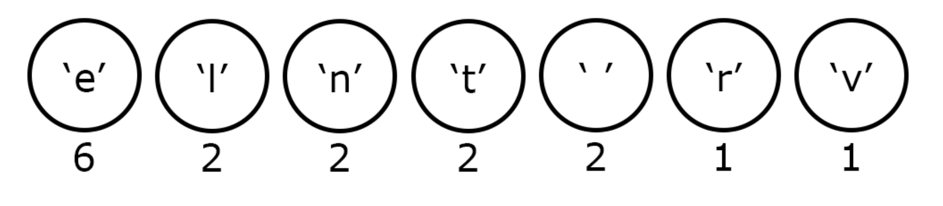
\includegraphics[width=100mm]{img/literatuurstudie/huffman-stap-1.png}}
	\caption{Een voorbeeld van hoe het resultaat na stap 1 (\ref{sec:primitieve-technieken-voorbeeld-huffman-encoding-1}) van \gls{huffman-coding} er voor de zin “lennert eet veel” kan uitzien. De volgorde van bomen met eenzelfde frequentie mogen van plaats gewisseld worden.}
	\label{fig:huffman-stap-1}
\end{figure}
\FloatBarrier

\subsubsection{Huffman encoding stap 2: bomen samenvoegen}
\label{sec:primitieve-technieken-voorbeeld-huffman-encoding-2}
Als tweede stap moeten alle bomen samengevoegd worden tot één boom waarbij voorrang gegeven wordt aan diegene met het kleinste totaal van frequenties. Indien er evenveel frequenties zijn heeft diegene met de kleinste diepte voorrang.

Een voorbeeld van hoe het resultaat van deze stap er voor de zin “lennert eet veel” kan uitzien is te vinden op figuur \ref{fig:huffman-stap-2}.

\FloatBarrier
\begin{figure}[h!]
	\fbox{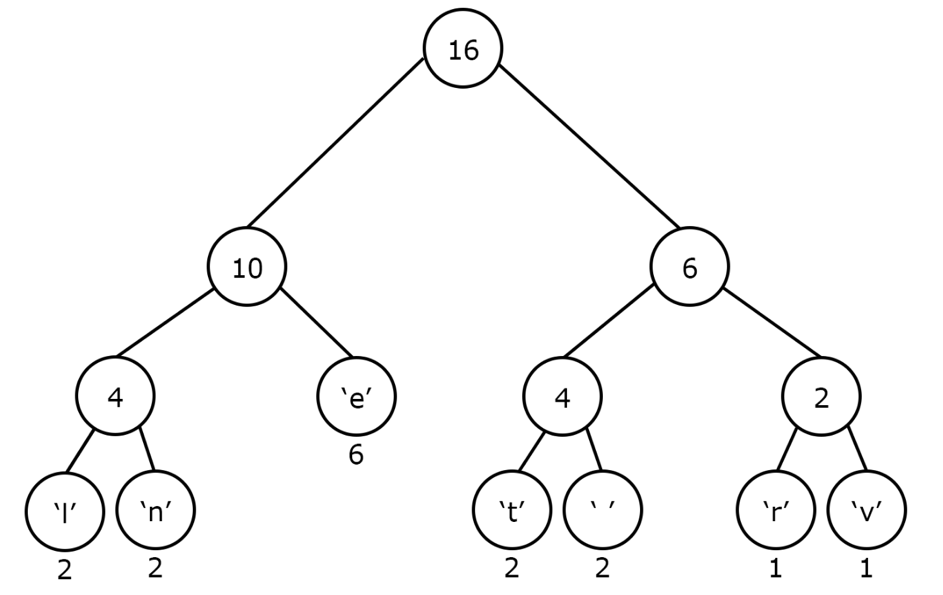
\includegraphics[width=100mm]{img/literatuurstudie/huffman-stap-2.png}}
	\caption{Een voorbeeld van hoe het resultaat na stap 2 (\ref{sec:primitieve-technieken-voorbeeld-huffman-encoding-2}) van \gls{huffman-coding} er voor de zin “lennert eet veel” kan uitzien. De knopen van een karakter met eenzelfde frequentie kunnen in sommige gevallen van plaats gewisseld worden.}
	\label{fig:huffman-stap-2}
\end{figure}
\FloatBarrier

\subsubsection{stap 3: prefix tabel (optioneel)}
\label{sec:primitieve-technieken-voorbeeld-huffman-encoding-3}
Als derde, optionele, stap kan voor elk karakter de \gls{prefix-code} gemaakt worden en bijgehouden worden in een \gls{lookup-table}. Dit wordt gedaan door het pad naar het blad van het karakter bij te houden startend uit het hoofd waarbij een stap naar links als 0 genoteerd wordt en een stap naar rechts als 1.

Het is ook mogelijk deze berekening van het pad steeds opnieuw te doen en dus geen gebruik te maken vaan een \gls{lookup-table}.

De bekomen binaire boom van stap \ref{sec:primitieve-technieken-voorbeeld-huffman-encoding-2} levert onderstaande \gls{lookup-table} op.

\FloatBarrier
\begin{table}[h!]
	\begin{tabular}{|l|l|}
		\hline
		\textbf{karakter} & \textbf{prefix} \\ \hline
		'e'               & 01              \\ \hline
		'l'               & 000             \\ \hline
		'n'               & 001             \\ \hline
		't'               & 100             \\ \hline
		' '               & 101             \\ \hline
		'r'               & 110             \\ \hline
		'v'               & 111             \\ \hline  
	\end{tabular}
\end{table}
\FloatBarrier

\subsubsection{stap 4: encoding}
\label{sec:primitieve-technieken-voorbeeld-huffman-encoding-4}
Als vierde en laatste stap kan nu eenvoudig weg elk karakter vervangen worden door zijn bijhorende \gls{prefix-code}. De zin “lennert eet veel” wordt door de bovenstaande \gls{lookup-table} voorgesteld als:
"000 01 001 001 01 110 100 101 01 01 100 101 111 01 01 000"

Het valt direct op dat deze reeks van \glspl{bit} (42 \glspl{bit}) veel kleiner is als in het \gls{ascii} voorbeeld (128 \glspl{bit}). Dit is de reden dat \gls{huffman-coding} tot op heden de grondlegger is voor veel \glspl{compressie-algoritme}. Hoewel \gls{huffman-coding} \gls{lossless} is en dus voornamelijk in andere \gls{lossless} \glspl{compressie-algoritme} gebruikt wordt is \gls{huffman-coding} ook te vinden als onderdeel van tal van \gls{lossy} \glspl{compressie-algoritme}.


\subsubsection{Huffman decoding}
\label{sec:primitieve-technieken-voorbeeld-huffman-decoding}
De \gls{decoding} is visueel het eenvoudigst met behulp van de binaire boom door links en rechts te gaan afhankelijk van de bit. Bij het vinden van een blad is een karakter gevonden en kan recursief terug van het hoofd begonnen worden. Binnen het \gls{compressie-algoritme} zal een soort van \gls{lookup-table} gebruikt worden dat samen met het gecomprimeerd bestand dient opgeslagen te worden.

\subsubsection{Huffman coding Probleemstelling 1: binaire boom niet opgeslagen}
\label{sec:primitieve-technieken-voorbeeld-huffman-probleem-1}
In het voorgaande deel (\ref{sec:primitieve-technieken-voorbeeld-huffman-decoding}) is bewezen dat via de \gls{huffman-coding} reeks en de oorpsronkelijke binaire boom het oorspronkelijk bericht volledig terug kan opgehaalt worden (of via de \gls{lookup-table}). Er is echter enkel rekening gehouden met de \gls{huffman-coding} reeks voor het bepalen van de bestandsgrootte. Volgens die logica zou de originele binaire boom (of lookup table) dus niet opgeslagen worden en bijgevolg zou de originele tekst niet meer te reconstrueren zijn. Een soort \gls{lookup-table} zal dus ook moeten opgeslagen worden als \gls{meta-data}.


\subsubsection{Huffman coding Probleemstelling 2: gecomprimeerd bestand groter dan bron}
Zoals in probleemstelling \ref{sec:primitieve-technieken-voorbeeld-huffman-probleem-1} besproken is moet een soort \gls{lookup-table} bijgehouden worden als \gls{meta-data} voor het gecomprimeerd bestand. Dit veroorzaakt echter een volgend potentieel probleem .


Wanneer zowel de \gls{huffman-coding} reeks als de binaire zoekboom moeten opgeslagen worden bestaat de kans dat het gecomprimeerde bestand een grotere bestandsgrootte heeft als het oorspronkelijk (door \gls{ascii} encoded) bestand. De mogelijkheid dat een gecomprimeerd bestand groter is dan een niet gecomprimeerd bestand is wederkerend bij \gls{datacompressie} en \gls{lossless} compressie in het bijzonder.


\subsubsection{Huffman coding Probleemstelling 3: overlappende prefix codes}
\label{sec:primitieve-technieken-voorbeeld-huffman-probleem-3}
\label{sec:primitieve-technieken-voorbeeld-huffman-probleem-2}
Door het gebruik van een binaire boom waarbij elk karakter voorgesteld wordt door een blad is het onmogelijk om een \gls{prefix-code} te bekomen die het begin is van een andere \gls{prefix-code}. In dit geval zou namelijk een knoop zijn aangeduid en geen blad (karakter).

Vooraleer er gebruik gemaakt werd van een binaire boom voor het bepalen van de \glspl{prefix-code} en het maken van de \gls{lookup-table} was dit echter wel een probleem. Zo konden \glspl{prefix-code} als 00, 001 en 00100 gelijktijdig voorkomen wat voor een gecomprimeerd bestand zorgt dat nooit met 100\% zekerheid gedecomprimeerd kan worden.

\section{Lossless vs lossy datacompressie}
\label{sec:ontstaan-datacompressie-lossless-lossy}
Zoals in hoofdstuk \ref{ch:termen} gedefinieerd slaat \gls{lossless} en \gls{lossy} op een categorie voor \glspl{compressie-algoritme}.
Bij \gls{lossless} \gls{datacompressie} is er geen verlies van 'kwaliteit' terwijl dit bij \gls{lossy} \gls{datacompressie} geen garantie is.

Het besproken \gls{huffman-coding} principe valt onder \gls{lossless} \gls{datacompressie}. Immers, de originele boodschap (en eender welke vorm van input) is bit per bit reconstrueerbaar door het \gls{compressie-algoritme}, er gaat dus geen data verloren. Een bit per bit reconstrueerbare clone is echter geen garantie voor \gls{lossless} \glspl{compressie-algoritme} aangezien \gls{meta-data} en andere zaken die geen impact hebben op “kwaliteit” wel verloren kunnen gaan.

Een typische \gls{use-case} voor \gls{lossless} \gls{datacompressie} zijn tekstdocumenten, de eindgebruiker wilt namelijk niet dat na het comprimeren letters verloren gaan in het document. 

Zoals reeds besproken in deel \ref{sec:ontstaan-datacompressie-primitieve-technieken-binnen-it} was de doorbraak van \gls{lossy} \gls{datacompressie} de opkomst van digitale afbeeldingen en muziek. Zo behoudt MP3 (\gls{lossy} \gls{codec} voor audio) bepaalde (combinaties van) audiofrequenties niet omdat die door het menselijke oor niet waarneembaar zijn. Maar ook waarneembare frequenties kunnen door de MP3 \gls{codec} verloren gaan voor het besparen van data. \gls{jpeg} is één van de oudste en bekendste vormen van \gls{lossy} \gls{compressie-algoritme} voor afbeeldingen. 

Zoals besproken in \citetitle{kaur2016} (\cite{kaur2016}) kunnen audiobestanden door het gebruik van \gls{lossy} \gls{datacompressie} tot 90\% kleiner worden in bestandsgrootte zonder een storende vermindering aan kwaliteit. Bij video kan een een nog grotere databesparing voorkomen, tot meer dan 99\% zonder daar veel visueel waarneembaar verschil mee gepaard gaat. Immers, opeenvolgende beelden lijken meestal erg op elkaar. Bij stilstaande afbeeldingen is het kwaliteitsverlies door \gls{lossy} \gls{datacompressie} vaak wel zeer zichtbaar wanneer 90\% of meer aan bestandsgrootte bespaard wordt.

De keuze voor \gls{lossless} of \gls{lossy} is \gls{use-case} gebonden. Bij het kiezen voor \gls{lossless} \gls{datacompressie} is een objectief onderzoek naar een goede balans tussen snelheid en databesparing voor de use case aangeraden. Bij \gls{lossy} \gls{datacompressie} zijn zowel objectieve als subjectieve onderzoeken mogelijk. In hoofdstuk \ref{ch:kwaliteit} wordt dieper ingegaan over de verschillende manieren om de prestatie van een \gls{compressie-algoritme} voor afbeeldingen te evalueren. In hoofdstuk \ref{ch:onderzoek} wordt een subjectief onderzoek gevoerd voor het bepalen van het geschikte \gls{afbeeldingsformaat} voor een bepaalde \gls{use-case}.


%deel 2
\chapter{Proof of concept compressietool}
\label{ch:compressietool}

In deel \ref{sec:primitieve-technieken-voorbeeld-rle} en \ref{sec:primitieve-technieken-voorbeeld-huffman-encoding} wordt uitgelegd hoe \gls{rle-long} en \gls{huffman-coding} werken. Dit hoofdstuk focust zich op de implementatie van deze \gls{compressie-algoritme}. Er zal een proof of concept \gls{compressietool} gebouwd worden in \gls{php} en de werking zal toegelicht worden. Deze is in staat om input bestanden onder de vorm van simpele tekst in een txt bestand om te zetten naar hen gecomprimeerde vorm.
 
\section{Gebruikte technologie}
\label{sec:compressietool-gebruikte-technologie}

Deze \gls{compressietool} is geschreven in \gls{php}. Dit maakt het mogelijk te tool eenvoudig lokaal te runnen door het gebruik van een webserver omgeving als \gls{xampp} of hem online te zetten op een \gls{hosting} platform. Deze tool is online raadpleegbaar op de website van Lennert Bontinck\urlcite{compressietool}.

\section{Run length encoding}
\label{sec:compressietool-rle}

TODO
%TODO: compressietool

\section{Huffman Coding}
\label{sec:compressietool-huffman}

TODO
%TODO: compressietool

\section{Patronen}
\label{sec:compressietool-patronen}

TODO
%TODO: compressietool

\section{Resultaten}
\label{sec:compressietool-resultaten}

TODO
%TODO: compressietool
%deel 3
\chapter{Afbeeldingcompressie}
\label{ch:afbeeldingcompressie}

%TODO: afbeeldingcompressie
\chapter{Videocompressie}
\label{ch:videocompressie}

\Gls{videocompressie} is een subdomein van \gls{datacompressie}. \Gls{videocompressie} bestaat er uit een video (verzameling van opeenvolgende afbeeldingen die frames genoemd worden) in zo weinig mogelijk aantal \glspl{bit} op te slaan terwijl een aanvaardbare kwaliteit behouden blijft. Dit kan zowel via \gls{lossless} als \gls{lossy} \glspl{compressie-algoritme}. \Gls{lossless} \gls{videocompressie} wordt in de praktijk echter zelden gebruikt voor web doeleinden door de grote hoeveelheid data dat ze in beslag nemen. \Gls{lossless} \gls{videocompressie} wordt vooral voor medische doeleinden gebruikt.

De output van een \gls{lossless} video \gls{codec} kan oplopen tot een bestand dat vijf tot wel twintig keer groter is dan een \gls{lossy} variant met een visueel zeer gelijkaardig resultaat. Een \gls{lossy} variant kan met enig verlies van kwaliteit meer dan 100 keer kleiner zijn dan een niet gecomprimeerde variant (\cite{importancelossyvidecodecs}). Het is door deze hoge \gls{compressieratio} dat de keuze voor een goede video \gls{codec} zo belangrijk is en dat het (live) streamen van video's mogelijk is. Zonder \gls{lossy} compressie zouden de meeste toestellen ook niet genoeg systeemresources hebben om de video vloeiend af te spelen.

De meest gebruikte \gls{lossy} video \glspl{codec} zijn \gls{h265} en motion \gls{jpeg2000}. Deze hebben beide ook een \gls{lossy} modus. De \gls{lossy} modus van \gls{h265} wordt in dit hoofdstuk besproken. Er wordt in deze bachelorproef niet verder ingegaan op \gls{lossy} video \glspl{codec}.

Dit hoofdstuk licht enkele van de bekendste video \glspl{codec} toe die grootschalig gebruikt worden door websites als YouTube en Netflix.

\section{Intra vs inter frame}
\label{sec:videocompressie-intra-inter}

\Gls{inter-frame} en \gls{inter-frame} \gls{datacompressie} zijn technieken voor \gls{videocompressie} dat gezamenlijk of individueel gebruikt kunnen worden door een video \gls{codec}. Dit kan volledig \gls{lossless} of \gls{lossy} gebeuren.

\Gls{intra-frame} \gls{datacompressie} kan het beste vergeleken worden met de compressie die binnen een \gls{afbeeldingsformaat} gebeurd. Het is een \gls{compressie-algoritme} dat één alleenstaand \gls{frame} comprimeert met enkel de data die het heeft van dat \gls{frame}. Dit kan bijvoorbeeld door \gls{pixel-prediction} (zoals \gls{png} besproken in deel \ref{sec:afbeeldingscompressie-png-werking}). Het is niet ongewoon dat alleenstaande \glspl{afbeeldingsformaat} gebruikt worden voor \gls{intra-frame} compressie. \Gls{jpeg2000} wordt vaak gebruikt voor videobestanden waar kwaliteit een grote rol spelen (in zijn \gls{lossless} of \gls{lossy} variant). Tegenwoordig is echter de omgekeerde verschijning meer voorkomend, dat \glspl{compressie-algoritme} oorspronkelijk gebruikt voor \gls{intra-frame} \gls{videocompressie} overgezet worden naar alleenstaande \glspl{afbeeldingsformaat}. Denk hierbij aan \gls{webp} dat van \gls{vp8}, een voorganger van \gls{av1} afkomstig is. \Gls{heic} komt oorspronkelijk ook uit \gls{intra-frame} \gls{datacompressie} bij \gls{h265}.

\Gls{inter-frame} \gls{datacompressie} maakt voor het comprimeren niet alleen gebruik van het huidige \gls{frame} maar ook voorgaande of volgende \glspl{frame}. Zo is het mogelijk om bijvoorbeeld verwijzingen te behouden naar éénzelfde achtergrond binnen een videofragment overheen de \glspl{frame}. Het aantal \glspl{frame} waarnaar verwezen kan worden is afhankelijk van de gebruikte \gls{codec}. Aangezien videofragmenten vaak wederkerende elementen hebben (zoals de achtergrond) voor een langdurige periode kan deze vorm van \gls{datacompressie} voor enorme besparingen zorgen. 

Een probleem dat bij \gls{inter-frame} \gls{datacompressie} opduikt is wanneer een bestand dat gebruikt maakt van dit \gls{compressie-algoritme} achteraf bijgesneden wordt. De verwezen \glspl{frame} (of delen van het frame bij croppen) kunnen hierdoor verloren zijn waardoor het decoden faalt. Hoewel sommige video bewerkingsoftware hier rekening mee houd door de verwijzingen naar \glspl{frame} dat verwijderd gaan worden eerst te vervangen door de effectieve data, is dit geen garantie.


\section{Video codecs}
\label{sec:videocompressie-video-codecs}

In die hoofdstuk worden video \glspl{codec} besproken en geen \glspl{container}. Een \gls{container} is, zoals de naam doet vermoeden, een verpakking voor alle data die opslagen moet worden en eventuele metadata. Deze containers bepalen de \gls{extensie} van een bestand,  enkele gekende video \glspl{container} zijn: \gls{mp4}, \gls{avi} en \gls{mkv}. Bij video's slaat de \gls{codec} dus data op in een passende \gls{container}. Ook de ondertiteling en dergelijke zijn opgenomen in de \gls{container}.

Een \gls{codec}, de coder-decoder, is de technologie verantwoordelijk voor de \gls{encoding} en \gls{decoding} van een bestand dat gebruik kan maken van één of meerdere \glspl{compressie-algoritme}. In het geval van een video \gls{codec} is dit de technologie dat het videofragment omzet in een zo klein mogelijke collectie van \glspl{bit}.

\subsection{H.264-AVC}
\label{sec:videocompressie-h264-AVC}

\Gls{h264-avc}, waarbij AVC voor 'advanced video coding' staat, is een onderdeel van de \gls{mpeg-4} \gls{iso} standaard dat in deel tien van deze standaard voor het eerst toegelicht wordt. Één van de eerste edities van \gls{iso}/IEC 14496-10 is online raadpleegbaar\urlcite{h264avciso} en geeft een inzicht op de basis werking van deze video \gls{codec}.

\Gls{h264-avc} is aangekondigd in mei 2003 en is daarmee de oudste besproken video \gls{codec} in deze bachelorproef. Desondanks zijn leeftijd is het nog altijd één van de meest gebruikte video \glspl{codec} op het web en in het algemeen. Dit is te weiden aan de jarenlange verder ontwikkeling van de standaard. De huidige versie van de \gls{iso} standaard is momenteel versie 25 uit april 2017. Deze voegt documentatie over het gebruik van \gls{hlg} met \gls{h264-avc} toe. Een veel gebruikte \gls{hdr} standaard.

\Gls{h264-avc} is een uitbreiding op vorige standaarden van de \gls{mpeg-4} standaard dat onder andere de volgende belangrijke extra functionaliteit met zich meebrengt:

\begin{itemize}
	\item Multi-picture inter-picture prediction. Deze techniek bied tal van voordelen op voorgaande technieken. Het voornaamste is de mogelijkheid om tot wel 16 verschillende referentie \glspl{frame} te kunnen bijhouden voor het comprimeren van één \gls{frame}. In vorige (bekende) standaarden waren hooguit twee referentie \glspl{frame} mogelijk. Deze uitbreiding kan voor (veel) kwaliteitswinst en een (veel) hoger \gls{compressieratio} zorgen in tal van scenario's. Bijvoorbeeld bij een \gls{frame} waar een achtergrond bestaat uit een combinatie van de achtergronden van meerdere \glspl{frame}.
	
	\item Flexibelere interlace opties dat het mogelijk maken de kijker het gevoel te geven dat de \gls{frame-rate} twee keer hoger is dan ze werkelijk is door twee verschillende \glspl{frame} met elkaar te combineren.
	
	\item Tal van technieken die de \gls{decoder} geschikt maken om te werken met livestreams waar enkele \glspl{frame} soms verloren gaan.
\end{itemize}

\subsubsection{H.264-AVC: voordelen}
\label{sec:videocompressie-h264-AVC-voordelen}

\Gls{h264-avc} is een standaard die reeds jarenlang wereldwijde adoptie kent. Dit is te weiden aan ondere andere volgende voordelen:

\begin{itemize}
	
	\item Een \gls{compressieratio} tot meer dan dubbel dat van voorgangers als MPEG-2 (\cite{h264avcmpeg2kwaliteit}) voor dezelfde perceptuele kwaliteit. Dit zorgt resulteert in de bestandsgrootte en het \gls{bandbreedte} gebruik.
	
	\item Een grote ondersteuning zowel op vlak van input \gls{frame} \glspl{afbeeldingsformaat} voor de \gls{encoder} als in internetbrowsers. Enkel ondersteuning op de Opera Mini browser ontbreekt volgens de gegevens van caniuse\urlcite{h264caniuse}.
	
	\item Ondersteuning voor livestreams met tal van functies om \glspl{artefact} zoveel mogelijk te bestrijden.
	
	\item Achterwaartse compatibiliteit voor \glspl{codec} gebaseerd op H.263 en H.261.
	
\end{itemize}

\subsubsection{H.264-AVC: nadelen}
\label{sec:videocompressie-h264-AVC-nadelen}

\Gls{h264-avc} bied ook enkele nadelen, de voornaamste zijn:

\begin{itemize}
	
	\item Heeft meer systeemresources nodig dan voorgaande \glspl{codec} voor zowel het \gls{encoding} als \gls{decoding} proces. Dit kan tragere chipset moeilijkheden geven om een video tegen zijn volle \gls{frame-rate} af te spelen. Ook het streamen van meerdere \gls{h264-avc} encoded video's kan zijn tol eisen.
	
	\item \Gls{h264-avc} is een zeer complex \gls{compressie-algoritme} wat het moeilijk maakt om als derde partij extensies te voorzien.
	
	\item \Gls{h264-avc} is ontwikkeld in een tijdperk waar full HD (1920 x 1080 \glspl{pixel}) een zeer hoge resolutie was. De maximum ondersteunde resolutie van \gls{h264-avc} is dan ook maximaal 4096x2304 \glspl{pixel}. 4K (3840 x 2160 \glspl{pixel}) is dus nog net ondersteund maar hogere resoluties niet meer. De bestandsgrootte van een \gls{h264-avc} groeit ook aanzienlijk eens de resolutie boven full HD gaat wat het voor 4K streaming minder interessant maakt.
	
	\item \Gls{h264-avc} vereist complexe licenties, die bij een herziening in 2015 nog complexer zijn geworden, voor zowel \gls{encoding} en \gls{decoding}. Deze licenties moeten zowel betaald worden door de bedrijven die \glspl{encoder} en \glspl{decoder} voorzien (internetbrowsers, apps, ...) als diegene die video's publiek beschikbaar maken (DVD's, YouTube, ...). Dit is gebaseerd op de eenheden verkocht (bv: individuele software en video's) of op het aantal abonnees (bv: streaming diensten). Er is een minimum van 100 duizend gebruikers vooraleer licenties nodig zijn, daarna kan een licentie tot wel 20 cent per extra gebruiker zijn.
	
\end{itemize}

\subsubsection{H.264-SVC}
\label{sec:videocompressie-h264-SVC}

\Gls{h264-svc}, waarbij SVC voor 'scalable video coding' staat, is een extensie op de in deel \ref{sec:videocompressie-h264-AVC} besproken \gls{h264-avc} \gls{videocompressie} standaard. Zoals de naam doet vermoeden verbeterd \gls{h264-svc} de schaalbaarheid van \gls{h264-avc}.

\Gls{h264-avc} kan slecht in één resolutie geëncodeerd worden. Om de optie te voorzien een gebruiker te laten kiezen in welke resolutie deze de video wil bekijken was dus het maken van verschillende video bestanden nodig. Dit nam niet alleen meer tijd en bestandsruimte in dan één groot bestand hebben maar kwam ook nadelig uit wanneer er dynamisch tussen verschillende resoluties geswitcht wou worden bij bijvoorbeeld een variërende \gls{bandbreedte} tijdens het streamen.

\Gls{h264-svc} bied een oplossing door één bestand te kunnen gebruiken voor het weergeven van meerdere resoluties. Dit maakt het eerder besproken dynamisch switchen tussen resolutie afhankelijk van de \gls{bandbreedte} mogelijk. Iets cruciaal bij (live) streamen waar het niet altijd mogelijk is een cache te maken en dus bij een tekort aan \gls{bandbreedte} geswitcht kan worden naar een lagere resolutie om te alle tijden 'iets' aan de eindgebruiker te kunnen laten zien. Hiervoor was zowel binnen hardware als software extra functionaliteit nodig op zowel netwerk als \gls{codec} laag. Een uitgebreid artikel over \gls{h264-svc} is \citetitle{H264svcoverview} (\cite{H264svcoverview}).


\subsection{H.265/HEVC}
\label{sec:videocompressie-h265}

\Gls{h265} is de officiële opvolger van \gls{h264-avc} dat het eerst is voorgesteld in april 2013. Het zorgt voor een bestandsgrootte dat gemiddeld 25 tot 50\% kleiner is dan \gls{h264-avc} met visueel gelijkaardige kwaliteit (\cite{h262h264h265vergelijking}). De gebruikte \gls{inter-frame} \gls{datacompressie} is de basis voor \gls{heif} besproken in deel \ref{sec:afbeeldingscompressie-heif}.

Een ander belangrijk voordeel van deze video \gls{codec} is dat het resolutie tot 8192×4320 \glspl{pixel} ondersteund, ongeveer het dubbele van zijn voorganger \gls{h264-avc}. \Gls{h265} ondersteund dus nog net 8K UHD waardoor de eerste adoptie voornamelijk in cinema's plaats vond.

De werking van \gls{h265} is meer een uitbreiding op \gls{h264-avc} dan een compleet nieuwe uitwerking. De voornaamste aanpassingen waardoor extra efficiëntie kan bereken worden zijn:

\begin{itemize}
	
	\item Een verbeterd \gls{inter-frame} \gls{compressie-algoritme} dat de basis legt voor \gls{heif}.
	
	\item Ondersteuning voor een groter vlak (64x64 \glspl{pixel} in plaats van 16x16 \glspl{pixel}) voor patroon compressie en difference-coding.
	
	\item Een betere \gls{compressie-algoritme} voor het gokken van een \gls{pixel} (\gls{pixel-prediction}) door een betere kennis van de camera beweging en hoe een \gls{pixel} zich verplaatst tegenover het voorgaande en volgende \glspl{frame}.
	
\end{itemize}

Hoewel \gls{h265} nog complexer is dan zijn voorganger \gls{h264-avc}, heeft dit voornamelijk impact op de \gls{encoding} tijd en niet zo zeer op de \gls{decoding} tijd. In 2014 zijn in een tweede revisie extensies toegevoegd voor schaalbaarheid.

\subsubsection{H.265/HEVC: voordelen}
\label{sec:videocompressie-h265-voordelen}

De voornaamste voordelen bij het gebruik van \gls{h265} over \gls{h264-avc} zijn:

\begin{itemize}
	
	\item Ondersteuning voor resoluties tot 8192×4320 \glspl{pixel}, waar 8K UHD net bijhoort.
	
	\item Gemiddeld besparing van 25 tot 50\%  ten opzichte van \gls{h264-avc} met een visueel gelijkaardige kwaliteit (\cite{h262h264h265vergelijking}).
	
\end{itemize}

\subsubsection{H.265/HEVC: nadelen}
\label{sec:videocompressie-h265-nadelen}

De voornaamste nadelen bij het gebruik van \gls{h265} zijn:

\begin{itemize}
	
	\item Complexe licenties zoals zijn voorganger \gls{h264-avc} die sterk kunnen oplopen, tot meer dan twintig keer zo duur als \gls{h264-avc}.
	
	\item Relatief slechte browser support enkel volledige ondersteuning op recente versies van iOS Safari en gedeeltelijke ondersteuning op Safari voor macOS, Internet Explorer en Edge.
	
	\item Een (veel) langere \gls{encoding} en iets langere \gls{decoding} tijd dan \gls{h264-avc} door te toegevoegde complexiteit.
	
\end{itemize}

\subsection{AV1}
\label{sec:videocompressie-av1}

\Gls{av1} is \gls{open-source} en royalty-free video \gls{codec} dat komaf maakt met de complexe en dure licenties verbonden aan andere video \glspl{codec} zoals \gls{h264-avc} en \gls{h265}. Het is ontwikkeld door AOMedia (Alliance for Open Media). Na een aankondiging in september 2015, samen met de opstart van AOMedia, is de eerste versie vrijgegeven in maart 2018 waarbij het ook het eerste project van AOMedia was.

AOMedia is een bedrijf van Google, Amazon, Netflix, Microsoft, Mozilla, Intel en Cisco. Grote bedrijven die een oplossingen wouden bieden tegen de problemen met de licenties van de voorgaande besproken video \glspl{codec}. Hoewel AOMedia een non-profit is hebben deze bedrijven er financieel baat bij dat \gls{av1} doorgroeid naar de standaard voor \gls{videocompressie}. Op die manier doen ze een immense besparing op licenties.

\Gls{av1} is gebaseerd op VP9, wat op zijn beurt gebaseerd is op \gls{vp8} en wiens \gls{inter-frame} \gls{compressie-algoritme} de basis legde voor het \gls{webp} \gls{afbeeldingsformaat}. De \gls{codec} begon zjin ontwikkeling als VP10 maar Google besloot het project over te plaatsen naar een afzonderlijk non-profit bedrijf om de redenen die hierboven reeds beschreven zijn.

Het vecht momenteel tegen \gls{h265} om de nieuwe standaard video \gls{codec} te worden.

\subsubsection{AV1: voordelen}
\label{sec:videocompressie-av1-voordelen}

\Gls{av1} is een zeer belovende video \gls{codec} en bied tal van voordelen. De voornaamste zijn:

\begin{itemize}
	
	\item Gratis in gebruik en makkelijk in implementatie door zijn \gls{open-source} en royalty-free eigenschap.
	
	\item Een vergelijkbaar of beter \gls{compressieratio} dan \gls{h265}.
	
	\item Een betere internetbrowser ondersteuning dan \gls{h265} door de relaties met Google en Mozilla. Een volledig overzicht wordt gegeven in deel \ref{sec:videocompressie-ondersteuning}.
	
	\item Meerdere 'levels' die het mogelijk maken om ondersteuning voor een hogere resolutie of \gls{frame-rate} toe te voegen. De huidige maximale resolutie is 7680 x 4320 \glspl{pixel} met een \gls{frame-rate} van 120 \glspl{frame} per seconde.
	
\end{itemize}

\subsubsection{AV1: nadelen}
\label{sec:videocompressie-av1-nadelen}

Ten opzichte van \gls{h265} heeft \gls{av1} maar één noemenswaardige nadeel buiten de ondersteuning die nog niet optimaal is doordat de \gls{codec} nog niet zo lang uit is. Het ondersteund nog geen realtime \gls{encoding} waardoor livesreaming met \gls{av1} op het moment van schrijven nog niet mogelijk is.

\Gls{av1} heeft echter wel reeds een betere ondersteuning dan \gls{h265} (op vlak van internetbrowsers), heeft geen complexe licenties en heeft een gelijkaardige \gls{encoding} en \gls{decoding} tijd ten opzichte van \gls{h265}.  

\section{De juiste keuze}
\label{sec:videocompressie-keuze}

De keuze voor een juiste video \gls{codec} is zeer \gls{use-case} gebonden en de juiste beslissing gaat gepaard met een goede keuze van de gebruikte audio \gls{codec} en \gls{container}. Verder onderzoek is hier dus aangeraden. De overzichten voor functionaliteit in deel \ref{sec:videocompressie-functies}, ondersteuning bij internetbrowsers in deel \ref{sec:videocompressie-ondersteuning} en op met betrekking tot licenties in deel \ref{sec:videocompressie-licentie} kunnen als startreferentie gebruikt worden.

\subsection{Functievereisten}
\label{sec:videocompressie-functies}

Het is belangrijk om voor elke \gls{use-case} grondig na te denken welke video \gls{codec} de beste keuze is. De selectie verfijnen kan je reeds eenvoudig doen door naar enkele functievereisten te kijken. Een korte overzichtstabel van enkele kernfunctionaliteiten per besproken video \gls{codec} is te vinden in figuur \ref{tab:overzichtstabel-videoformaten-functies}.

\begin{table}[]
	\begin{tabular}{|l|l|l|l|l|}
		\hline
		\textbf{}                  & \textbf{H.264/AVC}          & \textbf{H.264/SVC}         & \textbf{H265/HEVC}         & \textbf{AV1}                         \\ \hline
		\textbf{Compressieratio}   & \cellcolor[HTML]{9B9B9B}+   & \cellcolor[HTML]{9B9B9B}+  & \cellcolor[HTML]{32CB00}++ & \cellcolor[HTML]{32CB00}++           \\ \hline
		\textbf{Betalend}          & \cellcolor[HTML]{CB0000}Ja  & \cellcolor[HTML]{CB0000}Ja & \cellcolor[HTML]{CB0000}Ja & \cellcolor[HTML]{32CB00}Nee          \\ \hline
		\textbf{Browsersupport}    & \cellcolor[HTML]{32CB00}+   & \cellcolor[HTML]{32CB00}+  & \cellcolor[HTML]{CB0000}-- & \cellcolor[HTML]{9B9B9B}-            \\ \hline
		\textbf{Realtime encoding} & \cellcolor[HTML]{32CB00}Ja  & \cellcolor[HTML]{32CB00}Ja & \cellcolor[HTML]{32CB00}Ja & \cellcolor[HTML]{CB0000}Nee          \\ \hline
		\textbf{Schaalbaar}        & \cellcolor[HTML]{CB0000}Nee & \cellcolor[HTML]{32CB00}Ja & \cellcolor[HTML]{32CB00}Ja & \cellcolor[HTML]{32CB00}Ja           \\ \hline
		\textbf{Maximum resolutie} & \cellcolor[HTML]{CB0000}4K  & \cellcolor[HTML]{CB0000}4K & \cellcolor[HTML]{9B9B9B}8K & \cellcolor[HTML]{32CB00}Uitbreidbaar \\ \hline
	\end{tabular}
	\caption{Overzichtstabel van kernfunctionaliteit per video codec.}
	\label{tab:overzichtstabel-videoformaten-functies}
\end{table}

\subsection{Ondersteuning}
\label{sec:videocompressie-ondersteuning}

Een overzicht van de ondersteuning van de besproken video \glspl{codec} in de gekende internetbrowsers is beschikbaar in figuur \ref{tab:overzichtstabel-videoformaten-support}.

\begin{table}[]
	\begin{tabular}{|l|l|l|l|l|}
		\hline
		\textbf{}                   & \textbf{H.264/AVC}          & \textbf{H.264/SVC}          & \textbf{H265/HEVC}          & \textbf{AV1}                    \\ \hline
		\textbf{Chrome}             & \cellcolor[HTML]{32CB00}Ja  & \cellcolor[HTML]{32CB00}Ja  & \cellcolor[HTML]{CB0000}Nee & \cellcolor[HTML]{32CB00}Ja      \\ \hline
		\textbf{Edge}               & \cellcolor[HTML]{32CB00}Ja  & \cellcolor[HTML]{32CB00}Ja  & \cellcolor[HTML]{32CB00}Ja  & \cellcolor[HTML]{9B9B9B}Gepland \\ \hline
		\textbf{Firefox}            & \cellcolor[HTML]{32CB00}Ja  & \cellcolor[HTML]{32CB00}Ja  & \cellcolor[HTML]{CB0000}Nee & \cellcolor[HTML]{32CB00}Ja      \\ \hline
		\textbf{Safari}             & \cellcolor[HTML]{32CB00}Ja  & \cellcolor[HTML]{32CB00}Ja  & \cellcolor[HTML]{32CB00}Ja  & \cellcolor[HTML]{CB0000}Nee     \\ \hline
		\textbf{Internet explorer}  & \cellcolor[HTML]{32CB00}Ja  & \cellcolor[HTML]{32CB00}Ja  & \cellcolor[HTML]{32CB00}Ja  & \cellcolor[HTML]{CB0000}Nee     \\ \hline
		\textbf{Blackberry browser} & \cellcolor[HTML]{32CB00}Ja  & \cellcolor[HTML]{32CB00}Ja  & \cellcolor[HTML]{CB0000}Nee & \cellcolor[HTML]{CB0000}Nee     \\ \hline
		\textbf{Opera}              & \cellcolor[HTML]{32CB00}Ja  & \cellcolor[HTML]{32CB00}Ja  & \cellcolor[HTML]{CB0000}Nee & \cellcolor[HTML]{32CB00}Ja      \\ \hline
		\textbf{Opera Mini}         & \cellcolor[HTML]{CB0000}Nee & \cellcolor[HTML]{CB0000}Nee & \cellcolor[HTML]{CB0000}Nee & \cellcolor[HTML]{CB0000}Nee     \\ \hline
	\end{tabular}
	\caption{Overzichtstabel van internetbrowser ondersteuning per video codec. Data verkregen van caniuse.com in mei 2019.}
	\label{tab:overzichtstabel-videoformaten-support}
\end{table}

\subsection{Licenties}
\label{sec:videocompressie-licentie}

Op vlak van licenties is er maar één duidelijk winnaar: \gls{av1}. Deze \gls{codec} is \gls{open-source} en royalty-free waardoor de achterliggende code aangepast kan worden en gebruikt kan worden zonder een licentie te hoeven betalen. Een volledig overzicht van de licentievoorwaarden is te vinden op de website van AOMedia\urlcite{av1licenses}.

Licenties voor \gls{h264-avc}, \gls{h264-svc} en \gls{h265} zijn betalend en op aanvraag. Hoewel allen gratis zijn in gebruik onder een bepaalde grens is het aangeraden extra opzoekingswerk te verrichten voor de \gls{use-case} waarin deze \glspl{codec} zouden gebruikt worden.

\section{Implementatie}
\label{sec:videocompressie-implementatie}

De implementatie van video \glspl{codec} kan op een gelijkaardige manier als die van \glspl{afbeeldingsformaat}. Er zijn veelal \glspl{plug-in} beschikbaar om ondersteuning toe te voegen binnen videobewerkingssoftware dat de besproken \glspl{codec} standaard niet ondersteunen. Voor het implementeren op een webomgeving bestaan er net zoals bij \glspl{afbeeldingsformaat} besproken in deel \ref{sec:afbeeldingscompressie-implementatie} automatische en manuele oplossingen aan de hand van terugval video's of \gls{js} \glspl{decoder}. Deze implementaties zijn mede afhankelijk van de gekozen \gls{container} en audio \gls{codec} en worden daarom niet verder besproken in deze bachelorproef.
%deel 4
\chapter{Kwaliteit beoordelen}
\label{ch:kwaliteit}

TODO
%TODO: kwaliteit

\section{Objectieve beoordeling}
\label{sec:kwaliteit-objectief}

TODO
%TODO: kwaliteit

\section{Subjectieve beoordeling}
\label{sec:kwaliteit-subjectief}

TODO
%TODO: kwaliteit

\section{Instellingen voor kwaliteitsevaluatie}
\label{sec:kwaliteit-bedrijven}

TODO
%TODO: kwaliteit

\subsection{dxomark}
\label{sec:kwaliteit-dxomark}

TODO
%TODO: kwaliteit

\subsection{Maximum Compression}
\label{sec:kwaliteit-maximum-compression}

TODO
%TODO: kwaliteit

\subsection{Het probleem met deze instellingen}
\label{sec:kwaliteit-maximum-probleem}

TODO
%TODO: kwaliteit

\section{Tools voor kwaliteitsevaluatie}
\label{sec:kwaliteit-bedrijven}

TODO
%TODO: kwaliteit

\subsection{PSNR}
\label{sec:kwaliteit-psnr}

TODO
%TODO: kwaliteit

\subsection{SSIM}
\label{sec:kwaliteit-ssim}

TODO
%TODO: kwaliteit
\chapter{Onderzoek}
\label{ch:onderzoek}

Het kiezen voor een bepaald \gls{compressie-algoritme} is zeer \gls{use-case} gebonden. Zeker binnen \gls{videocompressie} en \gls{afbeeldingscompressie} is dit het geval. Ligt de focus op een zo klein mogelijke bestandsgrootte of juist op het behouden van zo veel mogelijk kwaliteit binnen een bepaalde omgeving? Wordt er voor een \gls{lossless} of \gls{lossy} \gls{compressie-algoritme} gekozen?

Zoals besproken in hoofdstuk \ref{ch:kwaliteit} zijn er zowel objectieve als subjectieve onderzoeken die kunnen gevoerd worden om een gepast \gls{compressie-algoritme} te bepalen. In dit hoofdstuk wordt een subjectief onderzoek uitgevoerd voor het bepalen van een geschikt \gls{afbeeldingsformaat} binnen een bepaalde \gls{use-case}. De gebruikte \gls{afbeeldingsevaluatietool} is ontwikkeld voor deze bachelorproef en is \gls{open-source} en gratis in gebruik. De code is te vinden op de \gls{github} repository van deze bachelorproef\urlcite{githubbachelorproef}. Dit maakt het heel eenvoudig dit onderzoek te reproduceren of een gelijkaardig onderzoek uit te voeren met andere \glspl{afbeeldingsformaat} en/of voor een andere \gls{use-case}.

De gebruikte afbeeldingen zijn op aanvraag beschikbaar: info@lennertbontinck.com.

\section{Waarom een subjectief onderzoek}
\label{sec:onderzoek-waarom-subjectief}

Zoals besproken in hoofdstuk \ref{ch:kwaliteit} is een subjectief onderzoek aangeraden binnen tal van \glspl{use-case}. Zeker binnen visuele \gls{datacompressie} kan dit de aangeraden manier van werken zijn aangezien de kwaliteit van de afbeeldingen een grote invloed heeft op de gebruikerservaring. 

Een objectief onderzoek dat bijvoorbeeld werkt aan de hand van het vergelijken van een afbeelding voor en na compressie kan een vals positief of negatief beeld geven over een bepaald \gls{afbeeldingsformaat}.

\section{Use case}
\label{sec:onderzoek-use-case}

De \gls{raw} bestanden gebruikt binnen dit onderzoek zijn aangeleverd door Mayté Bogaert van MaytéB fotografie. Aangezien zij ook aan het plannen is een online portfolio te bouwen vroeg ze zich af in welk \gls{afbeeldingsformaat} en met welke compressie instellingen ze de afbeelding het best online zet. Deze vraag is dan ook de \gls{use-case} van dit onderzoek.

Voor deze \gls{use-case} speelt de gebruikerservaring een zeer belangrijke rol. Als fotografe zijn afbeeldingen je product en moeten potentiële klanten deze dus positief ervaren wanneer ze op je portfolio terecht komen.

Langs de andere kant gaat het om een online website en moet er dus rekening gehouden worden met \gls{hosting} kosten, wachttijden en \gls{bandbreedte} gebruik. Als de website te lang duurt om te laden of alle mobiele data van een potentiële klant opgebruikt is dat geen goede reclame.

Er wordt dus een \gls{afbeeldingsformaat} gezocht met (zeer) goede beoordelingen uit het onderzoek dat de kleinste bestandsgrootte heeft.

\section{Afbeeldingsevaluatietool}
\label{sec:onderzoek-evaluatietool}

De gebruikte \gls{afbeeldingsevaluatietool} voor het voeren van dit onderzoek is een voor deze bachelorproef ontwikkelde \gls{afbeeldingsevaluatietool}. De code is te vinden op de \gls{github} repository van deze bachelorproef\urlcite{githubbachelorproef}. De \gls{afbeeldingsevaluatietool} is ook raadpleegbaar via de website van Lennert Bontinck\urlcite{evaluatietool}.

Deze tool is geschreven in \gls{php} met een achterliggende \gls{sql} databank. Er is een grafische interface voorzien die gebruik maakt van \gls{html}, \gls{css}, \gls{js}, \gls{jquery}, \gls{drift} en \gls{bootsrap}. Dit maakt het mogelijk de tool eenvoudig lokaal te runnen door het gebruik van webserver omgevingen als \gls{xampp} of online te plaatsen op de meeste \gls{hosting} platformen.

De \gls{afbeeldingsevaluatietool} maakt gebruik van een 50\% grijze achtergrond doorheen de ondervraging. Dit is de aangeraden kleur om geen impact te hebben op de perceptie van de kleuren binnen de afbeelding. Het inzoomen gebeurt aan de hand van pure \gls{js} waardoor geen manipulaties aan de afbeelding gebeuren en deze worden weergegeven zoals ze opgeslagen zijn. 

\subsection{Opzetten van de afbeeldingsevaluatietool}
\label{sec:onderzoek-evaluatietool-setup}

Een identiek onderzoek maar met andere afbeeldingen kan gevoerd worden zonder code aanpassingen te moeten uitvoeren wat de reproduceerbaarheid van dit onderzoek hoog houd. De gebruikte afbeeldingen kunnen ook op aanvraag geleverd worden, neem hiervoor contact via info@lennertbontinck.com.

Om de \gls{afbeeldingsevaluatietool} op te zetten clone je de \gls{github} repository. Alle nodige bestanden voor deze \gls{afbeeldingsevaluatietool} zijn te vinden onder de map 'evaluatietool'. Plaats alle bronbestanden uit deze map op de webserver en voorzie een database via localhost genaamd 'bachelorproef'. De gebruiker root met wachtwoord root moet toegang hebben tot deze database. 

De te evalueren afbeeldingen dienen voorzien te worden onder de map 'evaluatiereeks' en/of 'testreeks' te vinden in de map 'evaluatie\_afbeeldingen'.

Surf naar '/setup.php' en wacht tot er 'done' op het scherm verschijnt. De afbeeldingen zijn nu in de databank opgeslagen en het onderzoek is nu klaar om van start te gaan. Surf hiervoor naar '/index.php', je krijgt het welkomstscherm te zien zoals op figuur \ref{fig:bijlages-screenshot-afbeeldingsevaluatietool-welkom} weergegeven.

Aangezien bij dit onderzoek twee nog niet volledig ondersteunde \glspl{afbeeldingsformaat} worden getest, \gls{jpeg2000} en \gls{webp}, is een Apple computer met de Safari (voor \gls{jpeg2000}) en Google Chrome internetbrowsers (voor \gls{webp}) nodig. Het onderzoek begint in de Google Chrome internetbrowser en halverwege het onderzoek krijgt de deelnemer een scherm te zien dat deze moet overschakelen naar de Safari internetbrowser.

Voor het opzetten van de \gls{afbeeldingsevaluatietool} met extra functionaliteit zoals meer ondervraagde kenmerken of andere \glspl{afbeeldingsformaat} zijn aanpassingen van de code vereist. De code is in het volgende deel kort toegelicht en beschikt over verklarende functienamen en commentaar in de code zelf. 

\subsubsection{Afbeeldingsevaluatietool instellingen en uitbreidingen}
\label{sec:onderzoek-evaluatietool-setup-database}

\paragraph{Db/db\_actions.php}
\label{sec:onderzoek-evaluatietool-setup-db}

De database instellingen zijn bovenaan het bestand 'db/db\_actions.php' voorzien. De standaard waarden zijn in de code snippet hieronder weergegeven.

\begin{lstlisting}
$servername = "localhost";
$username = "root";
$password = "root";
$dbname = "bachelorproef";
\end{lstlisting}

In de functie 'create\_tables()' worden alle tabellen voorzien, deze wordt aangeroepen vanuit 'setup.php'. De volgende tabellen en velden worden reeds bijgehouden. In deze functie kunnen extra velden toegevoegd worden.

\begin{itemize}
	
	\item images
	\begin{itemize}
		\item image\_id $\rightarrow$ auto increment integer (primaire sleutel)
		\item filename $\rightarrow$ string 
		\item extension $\rightarrow$ string 
		\item path $\rightarrow$ string 
		\item practice\_data $\rightarrow$ boolean 
		\item chrome\_not\_safari $\rightarrow$ boolean
		\item filesize $\rightarrow$ integer
	\end{itemize}

	\item participants
	\begin{itemize}
		\item participant\_id $\rightarrow$ auto increment integer (primaire sleutel)
		\item gender $\rightarrow$ string 
		\item age $\rightarrow$ integer 
		\item expertise $\rightarrow$ boolean 
		\item colorblind $\rightarrow$ boolean 
		\item bad\_vision $\rightarrow$ boolean
	\end{itemize}

	\item ratings
	\begin{itemize}
		\item participant\_id $\rightarrow$ auto increment integer (samengestelde primaire sleutel)
		\item image\_id $\rightarrow$ auto increment integer (samengestelde primaire sleutel)
		\item sharpness $\rightarrow$ integer 
		\item color\_contrast $\rightarrow$ integer 
		\item general $\rightarrow$ integer
	\end{itemize}

\end{itemize}

Ook de overige database bewerkingen zijn te vinden in dit bestand. Dit zijn onder andere de functies voor het opslaan van de deelnemer zijn gegevens. Alle functies en variabelen hebben een verklarende benaming.

\paragraph{Js/*}
\label{sec:onderzoek-evaluatietool-setup-js}

In de folder 'js' is \gls{drift} voorzien onder het bestand 'drift.min.js'. In het bestand 'scripts.js' wordt een \gls{drift} instantie aangemaakt met de nodige instellingen. De standaard instellingen voor drift zijn hieronder zichtbaar. De zoom factor aanpassen kan door de waarde van 'zoomFactor' op de vijfde regel aan te passen.

\begin{lstlisting}[style=htmlcssjs]
if ($('.img_evaluation').length) {
	new Drift(document.querySelector('.img_evaluation'), {
		paneContainer: document.querySelector('.img_evaluation_zoomed'),
		inlinePane: 900,
		zoomFactor: 5,
		inlineOffsetY: -85,
		containInline: true,
		hoverBoundingBox: true,
		touchBoundingBox: true
	});
}
\end{lstlisting}

\paragraph{Layout/*}
\label{sec:onderzoek-evaluatietool-setup-layout}

In de folder 'layout' is de header en footer dat gedeeld wordt overheen de pagina's voorzien. De titel van de webpagina aanpassen of extra tags in de header voorzien kan in het bestand 'header.php'. De copyright in de footer veranderen of extra tags toevoegen op het einde van de webpagina kan in het bestand 'footer.php'.

\paragraph{Index.php}
\label{sec:onderzoek-evaluatietool-setup-index}

Het bestand 'index.php' verzorgt het welkomstscherm weergegeven in figuur \ref{fig:bijlages-screenshot-afbeeldingsevaluatietool-welkom}. In dit bestand kan u de welkomsttekst wijzigen. De knop onderaan de pagina bevat een verwijzing naar 'introductie.php'.

\paragraph{Introductie.php}
\label{sec:onderzoek-evaluatietool-setup-introductie}

Het bestand 'introductie.php' verzorgt de webpagina met de introductievideo weergegeven in figuur \ref{fig:bijlages-screenshot-afbeeldingsevaluatietool-video}. Het filmpje dat ingeladen wordt kan aangepast worden door een andere YouTube URL in te geven onder het src attribuut van regel twee of het pad naar een lokaal voorziene video.

\begin{lstlisting}[style=htmlcssjs]
<div class="embed-responsive embed-responsive-16by9">
	<iframe class="embed-responsive-item" src="https://www.youtube.com/embed/tqx-hmzO4kQ" allowfullscreen></iframe>
</div>
\end{lstlisting}

De knop onderaan deze webpagina verwijst naar 'onderzoek.php'

\paragraph{Onderzoek.php}
\label{sec:onderzoek-evaluatietool-setup-onderzoek}

Het bestand 'onderzoek.php' verzorgt de webpagina waar de deelnemer zijn informatie ingeeft en de afbeeldingen kan beoordelen weergegeven in figuur \ref{fig:bijlages-screenshot-afbeeldingsevaluatietool-over-u} en \ref{fig:bijlages-screenshot-afbeeldingsevaluatietool-evalutie}.  

In dit bestand wordt zijn volgende functies opgenomen met een verklarende naam:

\begin{itemize}
	\item show\_info\_about\_you()
	\item save\_info\_about\_you\_and\_show\_chrome()
	\item show\_start\_chrome\_sequence(\$participant\_id)
	\item show\_next\_iterative\_photo\_rating\_chrome()
	\item show\_photo\_rating(\$image\_id, \$path)
	\item save\_post\_rating\_image()
	\item show\_start\_safari\_sequence()
	\item show\_next\_iterative\_photo\_rating\_safari()
	\item show\_thanks\_screen()
\end{itemize}

\paragraph{Setup.php}
\label{sec:onderzoek-evaluatietool-setup-setup}

Het bestand 'setup.php' maakt de \gls{afbeeldingsevaluatietool} klaar voor gebruik. Hier worden de tabellen eerst verwijderd indien ze bestaan waarna ze terug aangemaakt worden. Vervolgens wordt elke afbeelding in de tabel 'images' gezet door de code hieronder voorzien.

\begin{lstlisting}
foreach (glob('evaluatie_afbeeldingen/testreeks/*.*') as $path) {
	$extension = pathinfo($path, PATHINFO_EXTENSION);
	$filename = pathinfo($path, PATHINFO_FILENAME);
	$chrome_not_safari = ($extension == "jpg" || $extension == "webp") ? 1 : 0;
	$practice_data = 1;
	$filesize = filesize($path);
	create_image_record($filename, $extension, $path, $practice_data, $chrome_not_safari, $filesize);
}
\end{lstlisting}

Op regel vier wordt bepaald of de afbeelding in Google Chrome moet weergegeven worden. Dit is het geval wanneer de \gls{extensie} die voor \gls{jpeg} of \gls{webp} is. Een gelijkaardig lus wordt gebruikt voor de evaluatiereeks. 

\paragraph{Export.php}
\label{sec:onderzoek-evaluatietool-setup-export}

Het bestand 'export.php' verzorgt de webpagina waar de organisator de geëxporteerde gegevens kan downloaden, weergegeven in figuur \ref{fig:bijlages-screenshot-afbeeldingsevaluatietool-export}.  

Voor het maken van de CSV bestanden wordt de volgende functie gebruikt.

\begin{lstlisting}
function make_csv_files() {
	//participants
	$file = fopen("temp/participants.csv", "w");
	fputcsv($file, array('participant_id', 'gender', 'age', 'expertise', 'colorblind', 'bad_vision'));
	$records = get_all_participants();
	while ($row = mysqli_fetch_assoc($records)) {
		fputcsv($file, $row);
	}
	fclose($file);
	
	//images
	...
	
	//ratings
	...
}
\end{lstlisting}

De volledige \gls{sql} tabel met de bijhorende velden worden dus gedumpt naar het CSV bestand met als heading de veldnamen. De code voor images en ratings is weggelaten omdat deze identiek is aan participants maar met andere variabelen namen.

\subsection{Verloop  van de afbeeldingsevaluatietool}
\label{sec:onderzoek-evaluatietool-verloop}

De \gls{afbeeldingsevaluatietool} is alomvattend voor het verzamelen van de gegevens omtrent dit onderzoek. Dit wil zeggen dat in de \gls{afbeeldingsevaluatietool} zelf beschreven wordt hoe de deze dient gebruikt te worden en welke gegevens van de deelnemer bewaart worden. De \gls{afbeeldingsevaluatietool} slaat ook alle input van de gebruiker automatisch op in de achterliggende \gls{sql} databank waardoor er geen manueel werk meer nodig is.

Enkele screenshots van de \gls{afbeeldingsevaluatietool} zijn raadpleegbaar in deel \ref{sec:bijlages-screenshot-afbeeldingsevaluatietool}.

\subsection{Verloop  van de afbeeldingsevaluatietool: Introductie}
\label{sec:onderzoek-evaluatietool-verloop-intro}

De deelnemer van het onderzoek wordt begroet met een scherm dat mededeelt waarover het onderzoek gaat, welke gegevens van de deelnemer gevraagd en bewaard zullen blijven en de geschatte duur van het onderzoek, zijnde een half uur tot drie kwartier. Een screenshot is voorzien in figuur \ref{fig:bijlages-screenshot-afbeeldingsevaluatietool-welkom}.

Als de deelnemer akkoord gaat met de gegevensverwerking wordt deze doorgebracht naar een volgende pagina met een introductievideo\urlcite{introductievideo} van 4 minuten op. Hierin worden de geëvalueerde onderdelen uitgelegd aan de hand van enkele extreme voorbeelden. Ook de \gls{use-case} en gegevensverwerking worden nogmaals uitgelegd. Een screenshot is voorzien in figuur \ref{fig:bijlages-screenshot-afbeeldingsevaluatietool-video}.

\subsection{Verloop  van de afbeeldingsevaluatietool: Informatie over deelnemer}
\label{sec:onderzoek-evaluatietool-verloop-info-participant}

Er worden enkele gegevens van de deelnemer gevraagd en opgeslagen zijnde: 

\begin{itemize}
	\item Geslacht (man, vrouw, overige)
	\item Leeftijd
	\item Of de deelnemer expertise heeft binnen het 
	onderzoeksdomein
	\item Of de gebruiker kleurenblind is
	\item Of de gebruiker slechtziend is
\end{itemize}

Het geslacht wordt bijgehouden om na te gaan om na te gaan of het mikpunt van 50/50 verhouding tussen man en vrouw bereikt is.

Een deelnemer wordt beschouwd als expertise hebbende wanneer deze een gegronde kennis heeft van \gls{afbeeldingscompressie} en \glspl{afbeeldingsformaat}, het verschil kent tussen \gls{lossless} en \gls{lossy} \glspl{compressie-algoritme} alsook artifacten zoals blokartifcaten kan herkennen in afbeeldingen.

Kleurenblindheid is een veelvoorkomend probleem bij mannen. Gemiddeld één op twaalf mannen heeft kleurenblindheid terwijl bij vrouwen dat gemiddelde onder de één op 250 ligt volgens \citetitle{porcella2008} (\cite{porcella2008}). Deze variabele wordt samen met slechtziendheid bijgehouden om na te gaan of dit een impact heeft op de perceptie van de afbeeldingen.

Een screenshot van dit scherm is voorzien in figuur \ref{fig:bijlages-screenshot-afbeeldingsevaluatietool-over-u}.

\subsection{Verloop  van de afbeeldingsevaluatietool: beoordeling}
\label{sec:onderzoek-evaluatietool-verloop-beoordeling}

Uiteindelijk krijgt de deelnemer voor elke afbeelding een evaluatiescherm te zien. Een screenshot van dit scherm is voorzien in figuur \ref{fig:bijlages-screenshot-afbeeldingsevaluatietool-evalutie}.

De volgorde van de afbeeldingen is voor elke deelnemer random bepaald. Indien er een testreeks voorzien is worden eerst de afbeeldingen uit deze testreeks aan de deelnemer getoond.

Op dit evaluatiescherm is aan de hand van \gls{drift} de mogelijkheid voorzien op de rechterhelft van het scherm een ingezoomde variant van de afbeelding op de linkerhelft te bekijken. Deze zoom is 5x en wordt bekomen door een pure \gls{js} oplossing. Dit wilt zeggen dat het originele bestand getoond wordt en er dus geen kwaliteitsverlies mogelijk is door deze \gls{plug-in}.

De deelnemer dient de afbeelding te beoordelen op de volgende drie kenmerken met een getal van één tot vijf:

\begin{itemize}
	\item Scherpte
	\item Kleuren en contrast
	\item Algemene indruk
\end{itemize}

\subsubsection{Kenmerk: scherpte}
\label{sec:onderzoek-evaluatietool-verloop-beoordeling-scherpte}

Een afbeelding wordt beschouwd als scherp wanneer de lijnen vloeiend worden weergegeven en er veel detail aanwezig is. Een fragment uit de introductievideo van de \gls{afbeeldingsevaluatietool} waarin het kenmerk scherpte wordt uitgelegd is terug te vinden in figuur \ref{fig:kenmerk-scherpte}.

\begin{figure}[]
	\centering
	\fbox{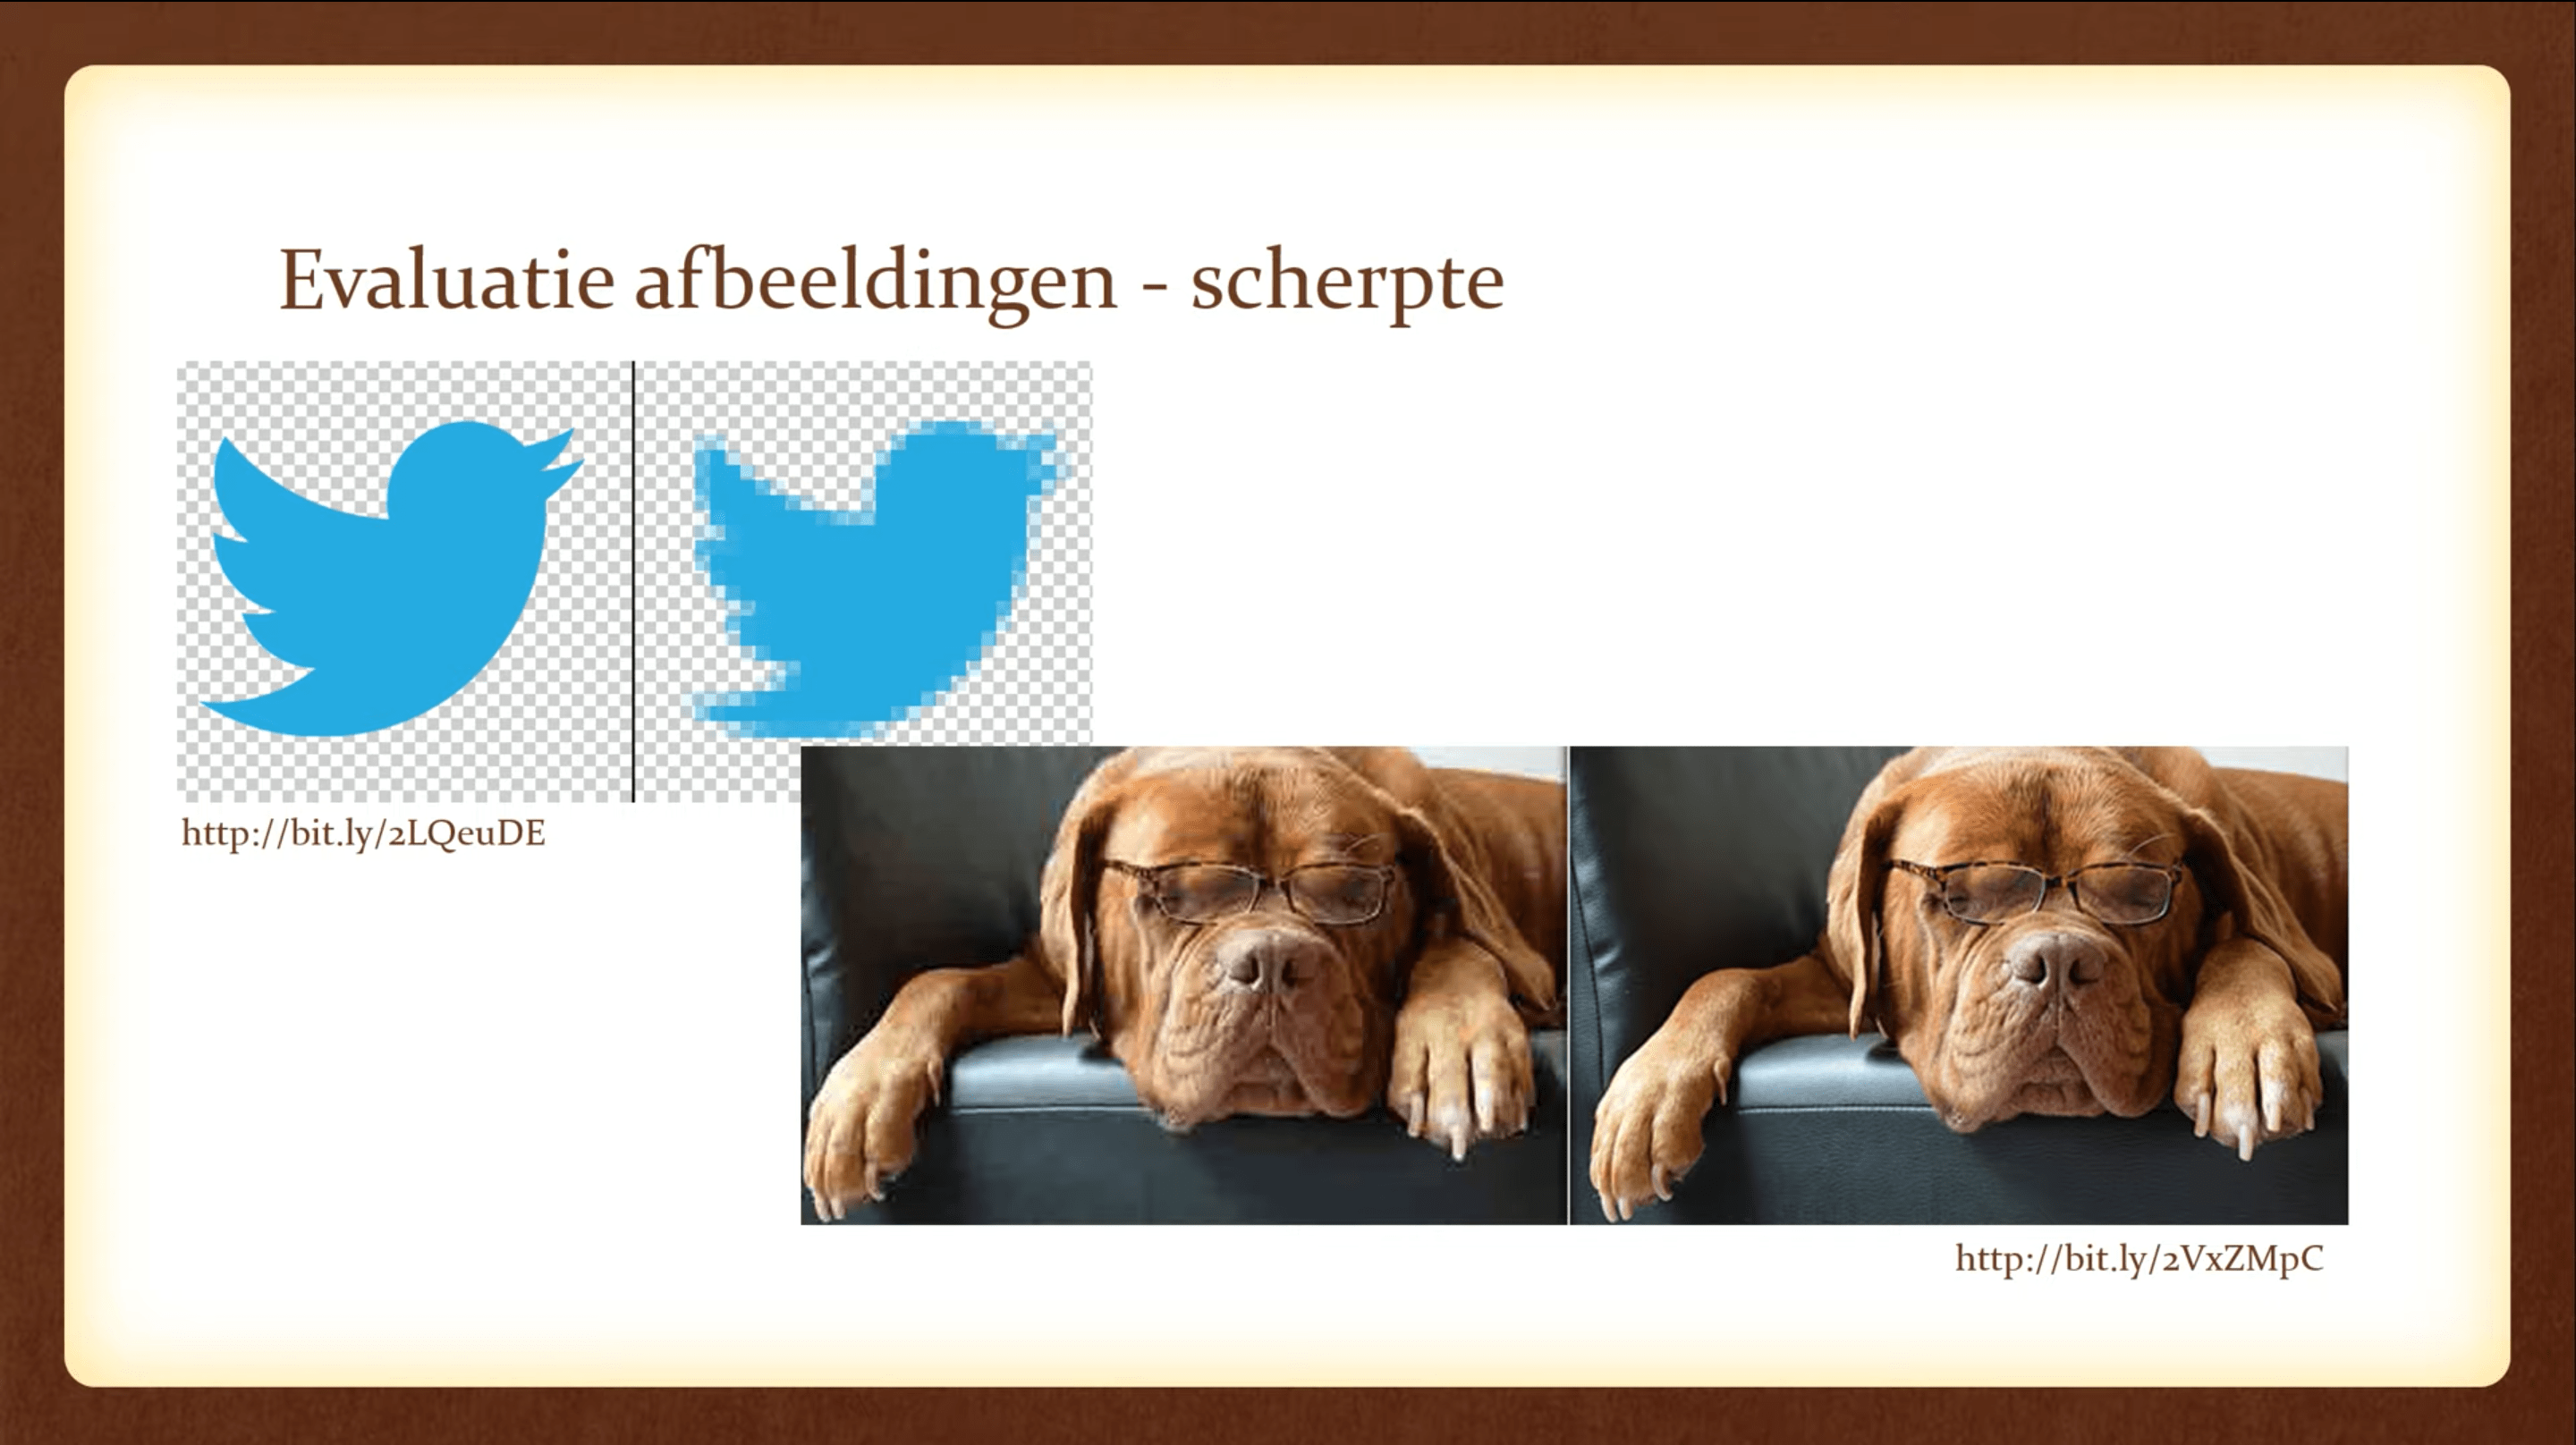
\includegraphics[width=0.6\linewidth]{img/onderzoek/scherpte.png}}
	\caption{Een fragment uit de introductievideo van de \gls{afbeeldingsevaluatietool} waarin het kenmerk scherpte (\ref{sec:onderzoek-evaluatietool-verloop-beoordeling-scherpte}) uitgelegd wordt. (\cite{introductievideo})}
	\label{fig:kenmerk-scherpte}
\end{figure}

Hier wordt scherpte uitgelegd aan de hand van van de randen in het Twitter logo links bovenaan waarbij de linkse variant zeer goed zou scoren (dus richting de vijf) en de rechter variant eerder slecht (richting de één).

Bij de hond is de linkerfoto de slechtere variant doordat veel detail rond de snuit verloren is gegaan. De hond heeft ook last van een slecht contrast op zijn poot waardoor bij de linker variant het verschil tussen de nagel en de poot soms slecht zichtbaar is.

\subsubsection{Kenmerk: kleuren en contrast}
\label{sec:onderzoek-evaluatietool-verloop-beoordeling-kleur}

Zoals hierboven besproken is de poot van de hond in figuur \ref{fig:kenmerk-scherpte} een goed voorbeeld van een slecht contrast. Op figuur \ref{fig:kenmerk-kleuren} is een fragment uit de introductievideo van de \gls{afbeeldingsevaluatietool} waarin het kenmerk kleur wordt uitgelegd zichtbaar. 

\begin{figure}[]
	\centering
	\fbox{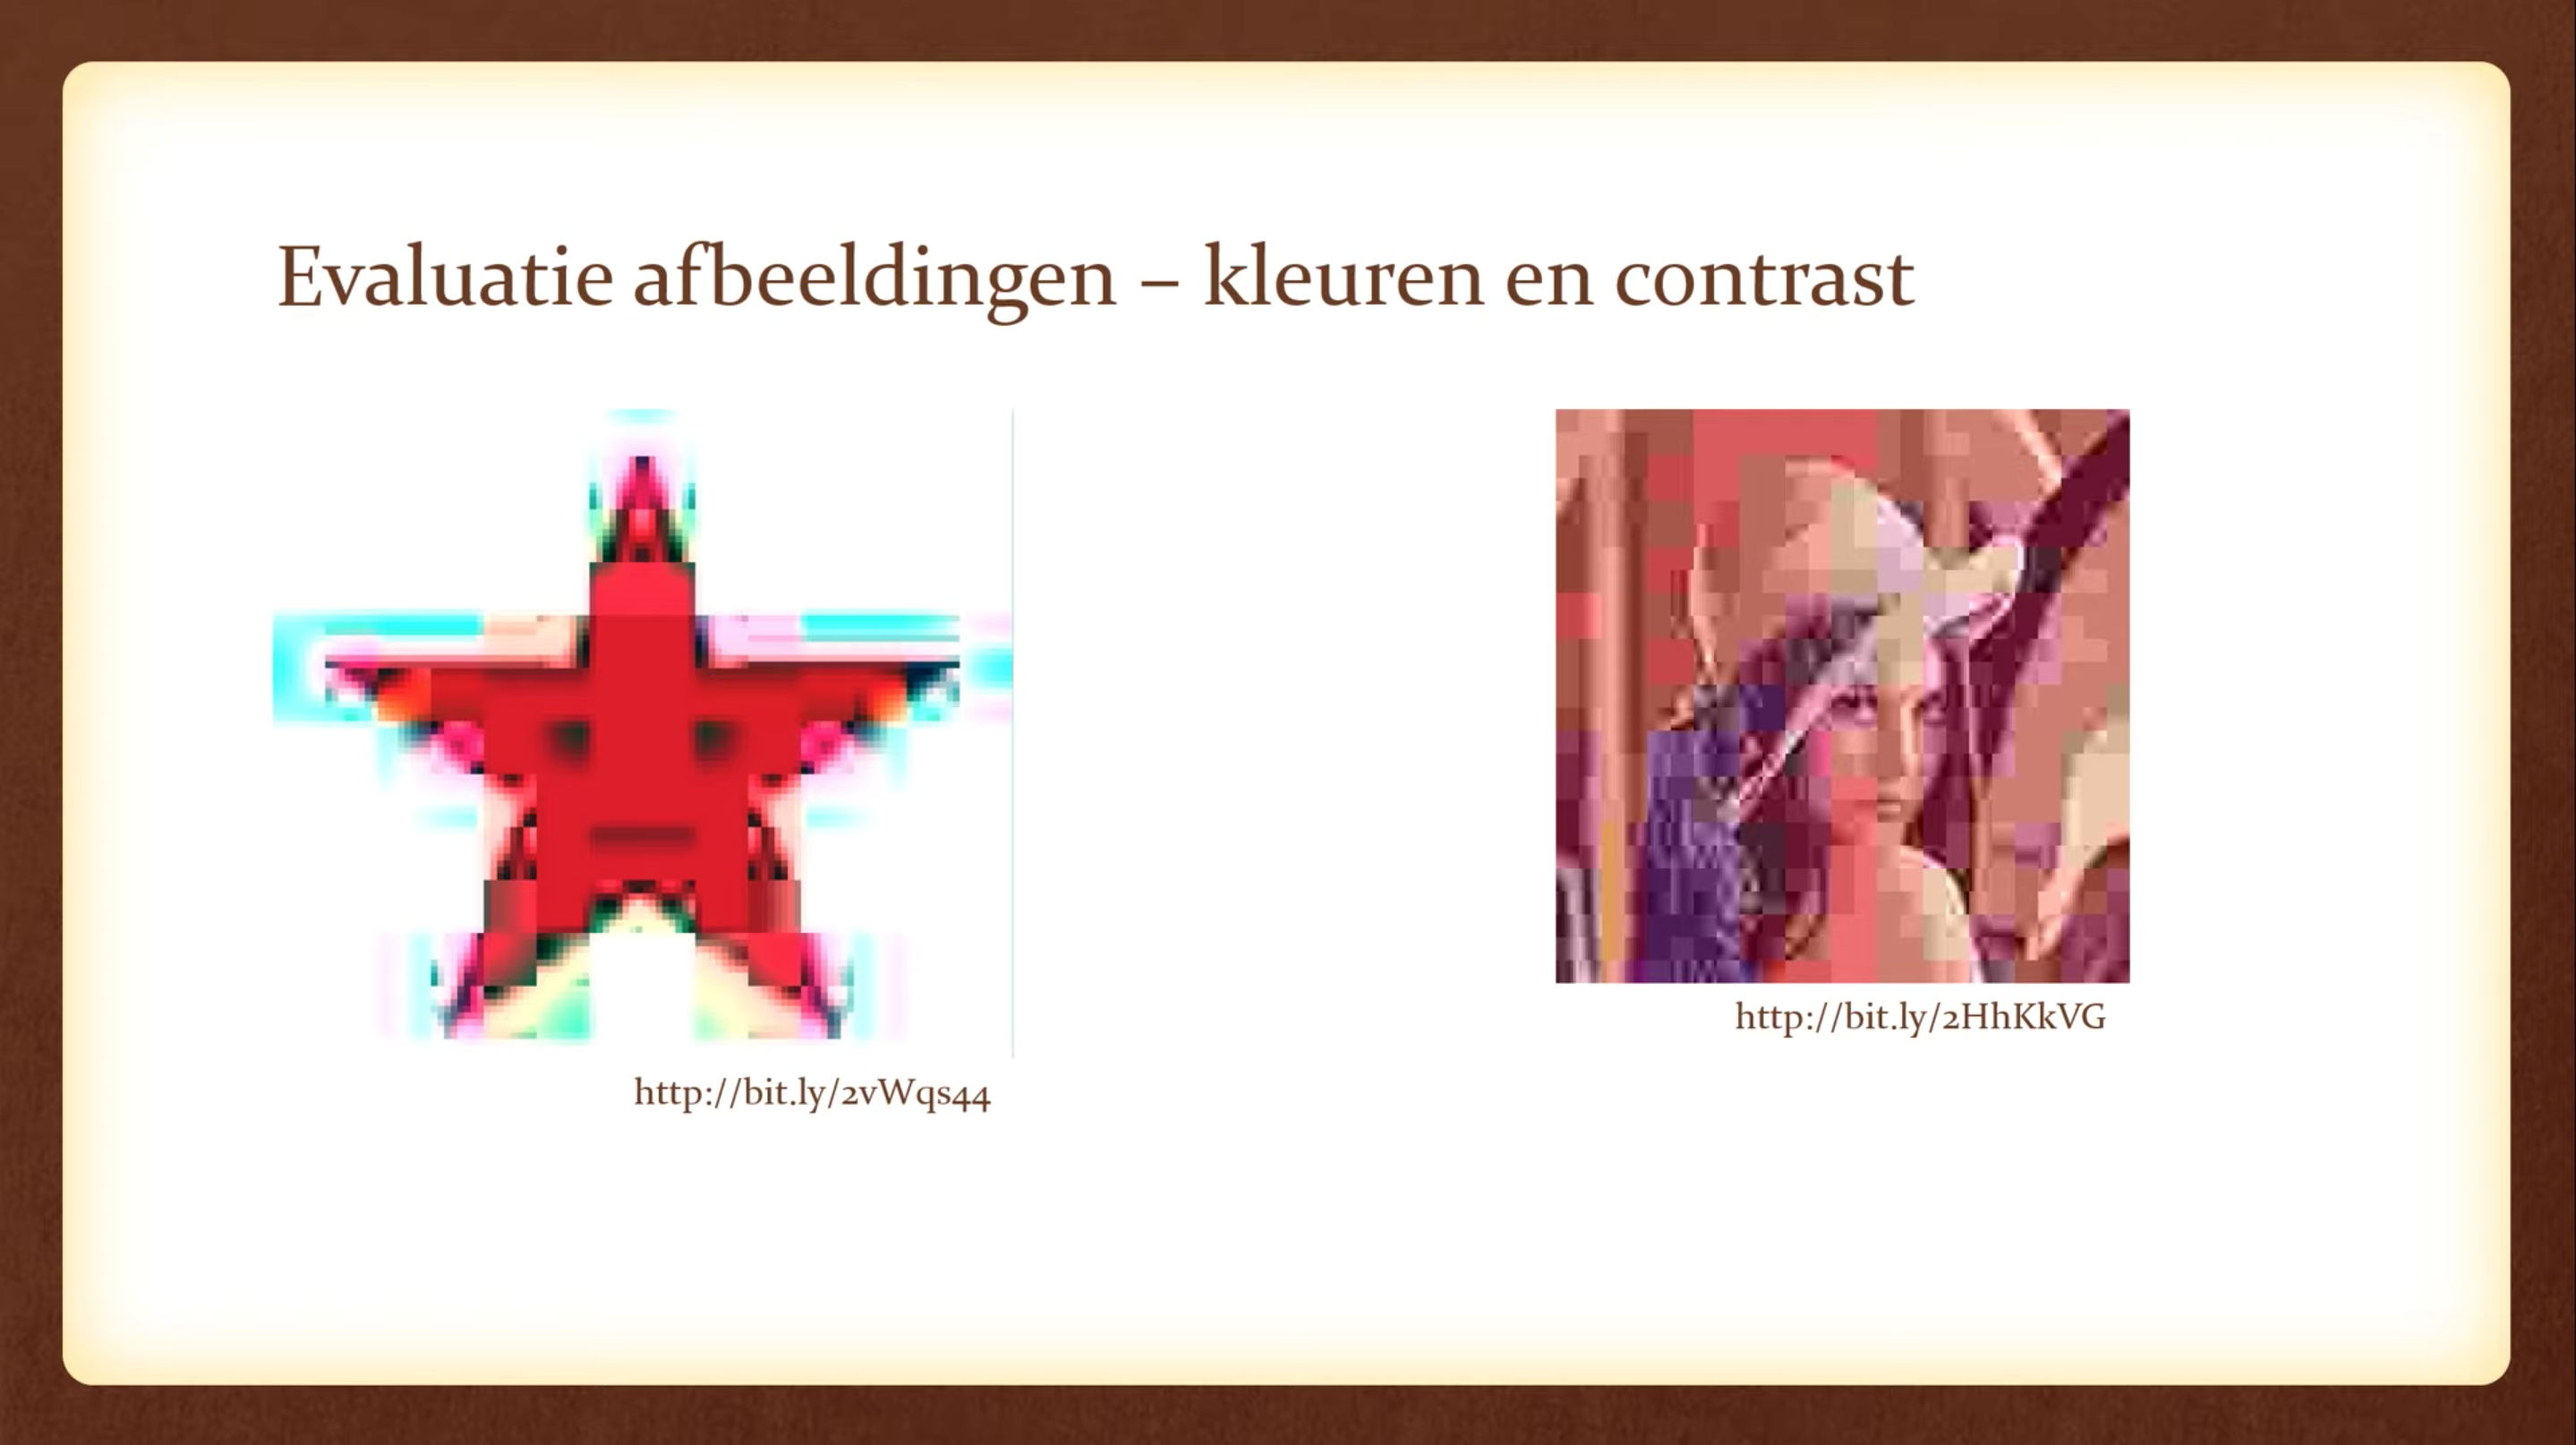
\includegraphics[width=0.6\linewidth]{img/onderzoek/kleuren.png}}
	\caption{Een fragment uit de introductievideo van de \gls{afbeeldingsevaluatietool} waarin het kenmerk kleuren en contrast (\ref{sec:onderzoek-evaluatietool-verloop-beoordeling-scherpte}) uitgelegd wordt. (\cite{introductievideo})}
	\label{fig:kenmerk-kleuren}
\end{figure}

Hier worden vooral veelvoorkomende soorten \glspl{artefact} met betrekking op kleur weergeven. Bijvoorbeeld de \glspl{artefact} zichtbaar bij de ster door clustering in bijvoorbeeld het \gls{jpeg} \gls{afbeeldingsformaat}.


\subsubsection{Kenmerk: algemene indruk}
\label{sec:onderzoek-evaluatietool-verloop-beoordeling-algemeen}

Tot slot wordt ook de algemene indruk van de deelnemer gevraagd omtrent deze afbeelding. Hier is het belangrijk dat de score geven wordt vanuit het standpunt dat de foto is tegenkomen op de portfolio van een fotografe zoals meegeven in de \gls{use-case} (deel \ref{sec:onderzoek-use-case}).

\subsection{Exporteren van de verzamelde gegevens}
\label{sec:onderzoek-evaluatietool-export}

Na het uitvoeren van het onderzoek kunnen de gegevens eenvoudig geëxporteerd worden naar drie verschillende CSV bestanden:

\begin{itemize}
	
	\item images.csv: een dump van de \gls{sql} tabel 'images' met als header de veldnamen.
	
	\item participants.csv: een dump van de \gls{sql} tabel 'participants' met als header de veldnamen.
	
	\item ratings.csv: een dump van de \gls{sql} tabel 'ratings' met als header de veldnamen.
\end{itemize}

Om deze CSV bestanden te genereren moet naar '/export.php' gesurft worden. Het export scherm, zichtbaar op figuur \ref{fig:bijlages-screenshot-afbeeldingsevaluatietool-export}, wordt weergegeven. De resultaten van dit onderzoek zijn beschikbaar op de \gls{github} repository van deze bachelorproef\urlcite{githubbachelorproef} onder de map 'resultaten'.

Het kan interessant zijn om de verschillende CSV bestanden samen te voegen naar één CSV bestand. Dit kaan eenvoudig in Python door gebruik te maken van Pandas. Het commando ziet er als volgt uit:

\begin{lstlisting}[language=Python]
import pandas as pd
images=pd.read_csv("/Users/lennertbontinck/Documents/github/bachelorproef-compressie/resultaten/csv/images.csv")
participants=pd.read_csv("/Users/lennertbontinck/Documents/github/bachelorproef-compressie/resultaten/csv/participants.csv")
ratings=pd.read_csv("/Users/lennertbontinck/Documents/github/bachelorproef-compressie/resultaten/csv/ratings.csv")
merged=images.merge(ratings,on="image_id")
merged=merged.merge(participants,on="participant_id")
merged.to_csv("/Users/lennertbontinck/Documents/github/bachelorproef-compressie/resultaten/csv/merged.csv", index=False)
\end{lstlisting}

De notebook voor het samenvoegen van de CSV bestanden is terug te vinden onder 'resultaten/python/merge/merge-csv.ipynb'.

Onder 'resultaten/python/*' zijn alle gebuikte notebooks voor het maken van de grafieken uit deel \ref{sec:onderzoek-resultaten}

\section{Uitvoering}
\label{sec:onderzoek-uitvoering}

Het onderzoek is gevoerd overheen twee maanden tijd waarbij in totaal 43 mensen hebben deelgenomen. Er wordt meer over de deelnemers gesproken in deel \ref{sec:onderzoek-uitvoering-deelnemers}. Het verloop van het onderzoek is te lezen in deel \ref{sec:onderzoek-evaluatietool-verloop}.

Voor de effectieve uitvoering van het onderzoek is met éénzelfde laptop gewerkt: een Apple MacBook Pro Mid 2014 15 inch met retina display. Dit toestel is gekozen voor zijn hoge resolutie scherm (2880x1800 \glspl{pixel}) een een goede representatie van het  sRGB color gamut. Bij elke deelnemer was verzekert dat de volgende zaken overeen kwamen:

\begin{itemize}
	\item Het testtoestel heeft 100\% batterij en is aangesloten op het netsnoer.
	
	\item Het testtoestel zijn helderheid staat op 100\% met alle vormen van kleuraanpassingen uitgeschakeld (night mode,...).
	
	\item Het testtoestel zijn toetsenbordverlichting staat uit zodanig dit niet voor reflectie in het scherm kan zorgen.
	
	\item Het testtoestel zijn scherm is volledig stof en vlek vrij gemaakt door het gebruik van een microvezeldoek.
	
	\item De gebruikte browsers staan klaar met leeggemaakte cache en in incognito modus zonder enige vorm van databesparing aan staat.
	
	\item De deelnemer zit in een door led lamp verlichte ruimte waarbij geen directe inval van zonlicht op het scherm is.
\end{itemize}

Op deze manier zijn zoveel mogelijk randvariabelen geëlimineerd bij het uitvoeren van het onderzoek.

De auteur van deze bachelorproef was ten alle tijden aanwezig in het onderzoek moesten er vragen zijn of er zich problemen voor doen.

\subsection{Geëvalueerde afbeeldingen}
\label{sec:onderzoek-uitvoering-afbeeldingsformaten}

Voor dit onderzoek zijn 15 afbeeldingen geëvalueerd in de volgende vier \glspl{afbeeldingsformaat}: 

\begin{itemize}
	\item \gls{png}
	
	\item \gls{jpeg}
	
	\item \gls{jpeg2000}
	
	\item \gls{webp}
\end{itemize}

Er is gebruik gemaakt van een selectie \gls{raw} afbeeldingen aangeleverd door Mayté Bogaert van MaytéB fotografie met volgende kenmerken:

\begin{itemize}
	\item Getrokken met een 'Nikon D750' toestel en 'TAMRON SP AF 28-75mm F2.8 XR Di LD Aspherical IF Macro A09NII' lens.
	
	\item Portretfoto's waarbij het onderwerp in focus is en de achtergrond wazig door het gebruik van een kleine diafragma waarde (grote opening).
	
	\item Zowel afbeeldingen die met en zonder flash genomen zijn.
	
	\item Zowel afbeeldingen die in een zeer goed verlichte omgeving als donkere omgeving genomen zijn.
	
	\item Zowel afbeeldingen met een groot contrast en een klein contrast.
\end{itemize}

De afbeeldingen zijn allen geëxporteerd vanuit \gls{ps}. Hiervoor is het steeds het \gls{raw} bestand als startbestand gebruikt waarbij de canvasgrootte omgezet is naar 1000 x 1498 \glspl{pixel} (portret) of 1498 x 1000 \glspl{pixel} (landschap). Het exporteren naar \gls{png}, \gls{jpeg}, en \gls{jpeg2000} zitten standaard ingebouwd in deze versie van \gls{ps} (CC 20.0.0). Voor het exporteren naar \gls{webp} is gebruik gemaakt van de gratis \gls{open-source} \gls{plug-in} 'AdobeWebM' door fnordware\urlcite{fnordwarewebm}.

De exacte instellingen gebruikt voor het opslaan van de afbeeldingen is terug te vinden in figuur \ref{fig:bijlages-onderzoek-render}.

\subsection{Deelnemers}
\label{sec:onderzoek-uitvoering-deelnemers}

In totaal hebben er 43 mensen deelgenomen aan het onderzoek waarvan 15 vrouwen en 28 mannen. Zes personen hebben opgegeven dat ze expertise binnen het domein hebben, drie mensen dat ze slechtziend zijn op het moment dat ze het onderzoek afleggen en twee personen hebben aangegeven dat ze kleurenblind zijn. Dit waren beide mannen. Deze gegevens komen overeen met de verwachting uit deel \ref{sec:onderzoek-evaluatietool-verloop-info-participant}. Hoewel er geen perfecte 50/50 verhouding is tussen mannen en vrouwen is deze verhouding aanvaardbaar.

Alle informatie die in dit deel benoemd is, is te bepalen via de Python scripts te vinden onder 'resultaten/python/statistieken/participants/*'. De gebruikte CSV is te vinden onder 'resultaten/csv/participants.csv'.

\section{Resultaten}
\label{sec:onderzoek-resultaten}

De resultaten zijn na afloop van het onderzoek geëxporteerd naar drie CSV bestanden en samengevoegd naar één CSV bestand zoals uitgelegd in deel \ref{sec:onderzoek-evaluatietool-export}. Alle informatie dat in dit deel toegelicht zal worden, is te bepalen via de Python scripts te vinden onder 'resultaten/python/statistieken/*'. De gebruikte CSV bestanden zjin te vinden onder 'resultaten/csv/*'.

\section{Resultaten lossless afbeeldingsformaten}
\label{sec:onderzoek-resultaten-lossles}

Zoals verwacht scoort \gls{png} en de \gls{lossless} variant van \gls{webp} en \gls{jpeg2000} zeer goed. In figuur \ref{fig:bijlages-onderzoek-resultaten-png-gem-med} is duidelijk te zien dat \gls{png} voor het kenmerk 'algemene indruk' steeds een mediaan heeft van vijf en het gemiddelde ook dicht bij vijf ligt, de maximumscore. Dit is ook voor kenmerk 'scherpte' en 'kleuren en contrast' het geval. Een bijna identiek resultaat is zichtbaar voor de \gls{lossless} variant van \gls{webp} (figuur \ref{fig:bijlages-onderzoek-resultaten-lossless-webp-gem-med}) en de \gls{lossless} variant van \gls{jpeg2000} (figuur \ref{fig:bijlages-onderzoek-resultaten-lossless-jpeg2000-gem-med}).

Wanneer echter naar de bestandsgrootte wordt gekeken is wel een groot verschil te zien tussen de verschillende \glspl{afbeeldingsformaat}. Dit wordt weergegeven in figuur \ref{fig:onderzoek-resultaten-lossless-sizes}. \Gls{webp} scoort in beide gevallen iets beter dan \gls{jpeg2000} welke, met behoorlijke marge, beter presteert dan \gls{png}.  

\begin{figure}[]
	\centering
	\fbox{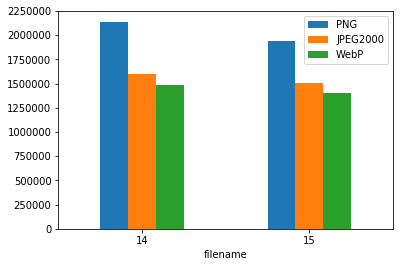
\includegraphics[width=0.5\linewidth]{img/bijlages/onderzoek/resultaat/lossless/lossless_sizes.png}}
	\caption{De bestandsgrootte in \glspl{bit} voor de afbeeldingen dat \gls{lossless} gecomprimeerd zijn door zowel \gls{png}, \gls{jpeg2000} en \gls{webp}.}
	\label{fig:onderzoek-resultaten-lossless-sizes}
\end{figure}

\section{Resultaten lossy afbeeldingsformaten}
\label{sec:onderzoek-resultaten-lossy}

Afbeelding één tot en met dertien zijn door \gls{jpeg}, \gls{jpeg2000} en \gls{webp} \gls{lossy} gecomprimeerd. De gebruikte instellingen zijn terug te vinden in figuur \ref{fig:bijlages-onderzoek-render}.

Wat direct opvalt is dat de bestandsgroottes immens verschillen desondanks percentuele instellingen voor kwaliteitsbehoud identiek waren. Dit is weergegeven in figuur \ref{fig:onderzoek-resultaten-lossy-sizes}. Dit maakt het moeilijk om de resultaten voor de \gls{lossy} \glspl{afbeeldingsformaat} te vergelijken. Het verschil in \gls{compressieratio} verschilt namelijk te sterk om per afbeelding de \glspl{afbeeldingsformaat} te vergelijken. 

Er kan echter wel een interessant overzicht gemaakt worden door een verhouding tussen de bestandsgrootte en toegekende scores op te stellen. Deze verhoudingen zijn weergegeven in figuur \ref{fig:onderzoek-resultaten-lossy-ratio-jpf}, \ref{fig:onderzoek-resultaten-lossy-ratio-jpg} en \ref{fig:onderzoek-resultaten-lossy-ratio-webp}. Als we deze figuren vergelijken met de figuren van de bestandsgrootte, en de verhoudingen vergelijken daar waar de bestandsgroottes gelijkaardig zijn, is \gls{webp} de duidelijke winner.

\section{Besluit}
\label{sec:onderzoek-besluit}

Hoewel de gegevens niet ideaal zijn door de onverwachts grote variatie in compressieratio tussen de \glspl{afbeeldingsformaat}, is er wel een duidelijke trend met de beschikbare gegevens. \Gls{webp} behaald voor een zelfde bestandsgrootte een aanzienlijke grotere score dan \gls{jpeg2000} wat op zijn beurt beter presteert dan \gls{jpeg}. Ook valt op dat de scores voor de drie kenmerken bij \gls{webp} zeer gelijkaardig zijn terwijl bij \gls{jpeg} en \gls{jpeg2000} de kleur gemiddeld gezien bij bijna alle afbeeldingen het slechtst scoort, gevolgd door de scherpte. De gegeven algemene score ligt gemiddeld gezien ook hoger dan zowel de score op scherpte als op kleuren en contrast voor de drie \glspl{afbeeldingsformaat}.

Zoals verwacht krijgen de \gls{lossless} \glspl{afbeeldingsformaat} zeer gelijkaardige scores. Dit is dan ook het kenmerk van \gls{lossless}, dat ze een afbeelding produceren zonder kwaliteitsverlies en dus identiek zijn ongeacht het \gls{afbeeldingsformaat}. Hier kan een winnaar dus puur objectief gekozen worden op basis van bestandsgrootte en ook daar wint \gls{webp}. \Gls{jpeg2000} is bij de geteste \gls{lossless} gecomprimeerde afbeeldingen tussen de vijf en tien percent groter dan \gls{webp}. \Gls{png} is aanzienlijk groter dan \gls{lossless} \gls{jpeg2000} en \gls{webp} met een bestandsgrootte van ongeveer 30\% meer dan de andere \glspl{afbeeldingsformaat}.

Voor deze \gls{use-case} kan dus besloten worden gebruik te maken van een manuele implementatie waarbij het picture element gebruikt wordt besproken in \ref{sec:afbeeldingscompressie-implementatie-web}. De volgorde voor ondersteuning is dan \gls{webp}, \gls{jpeg2000} en tot slot \gls{jpeg2000}. Deze afbeeldingen zullen manueel voorzien worden aangezien het gebruik van een \gls{js} \gls{decoder} een dubbele \gls{lossy} \gls{datacompressie} zou veroorzaken wat ongewenste kwaliteitsgevolgen kan hebben. Wanneer een bezoeker op een afbeelding klikt zal een \gls{lossless} \gls{webp} afbeelding geladen en vergroot getoond worden. Indien deze niet ondersteund wordt zal gebruik gemaakt worden van de \gls{js} \gls{decoder} om hem om te zetten naar \gls{png} zoals besproken in deel \ref{sec:afbeeldingscompressie-implementatie-web-automated}. Dit beperkt de overhead voor het creëren van de afbeelding in alle \glspl{afbeeldingsformaat} enigszins. Op Google I/O 2019 is echter ook een nieuwe feature van Google Chrome aangekondigd dat eenvoudig geïmplementeerd kan worden. Door het voorzien van de data tag loading=''lazy'' zal Google Chrome automatisch de afbeeldingen lazy loaden waardoor de gebruiker de webpagina reeds kan zien zonder de afbeeldingen ingeladen zijn. Dit bevorderd de response time enorm.
%deel 5
\chapter{Huidige en toekomstige uitdagingen}
\label{ch:uitdagingen}

In dit korte hoofdstuk zullen enkele huidige uitdagingen van \gls{datacompressie} toegelicht worden. Hiermee zal worden aangetoond dat \gls{datacompressie} een enorm groot begrip is dat veel verder gaat dan alleen \gls{afbeeldingscompressie} en \gls{videocompressie}.

\section{DNA compressie}
\label{sec:uitdagingen-dna-compressie}

Het menselijke DNA kan digitaal voorgesteld worden door een lange lijst van 5 verschillende karakters, gekend als basen. Deze digitale voorstelling bestaat uit meer dan 3 miljard van deze basen (\cite{dodanaugent2011}). DNA compressie bestaat er uit deze reeks van basen zo efficiënt mogelijk op te slaan zodanig performante bewerkingen mogelijk zijn met een zo klein mogelijke bestandsgrootte.

Hoewel met de huidige technologie en kennis reeds tal van informatie uit DNA gehaald kan worden, zal verdere uitwerkingen van \gls{dna-compressie} technieken het opslaan van een gigantische hoeveelheid DNA enkel bevorderen.  Dit kan op zijn beurt voor tal van andere doorbraken zorgen. Zo is een AI, die voorzien is van voldoende trainingsdata, mogelijks in staat relaties te vinden tussen DNA en bepaalde aandoeningen dat huidige wetenschappers momenteel niet vinden.

Vakexpert en co-promotor van deze bachelorproef, Tom Paridaens, houd zich op professionele basis bezig met \gls{dna-compressie}.

\subsection{AI en compressie}
\label{sec:uitdagingen-ai}

Zoals besproken in deel \ref{sec:uitdagingen-dna-compressie} is het door verdere databesparing mogelijk meer data te verzamelen en op te slaan. Deze grotere hoeveelheid aan data kan tot een stijging van beschikbare trainingsdata voor AI's zorgen. Dit is ten voordele van de werking van de AI.

Maar ook de bestanden die een AI genereert kunnen verdere \gls{datacompressie} gebruiken. Zo is in Google I/O 2019 besproken dat het model voor natuurlijke stem herkenning verkleind is van ongeveer honderd gigabyte naar nog geen één gigabyte. Dit maakt het mogelijk de modellen te voorzien op toestellen zelf in plaats van in de cloud. Dit wil niet alleen zeggen dat de diensten offline gebruikt kunnen worden maar ook dat de latency aanzienlijk kleiner wordt. 

Meer details over hoe deze verkleining bereikt is, is op het moment van schrijven nog niet beschikbaar maar er zal vermoedelijk gebruik gemaakt zijn van het selectief verwijderen van data aan de hand van een zeer complex \gls{lossy} \gls{compressie-algoritme}. Achterliggend zullen ook tal van \gls{lossless} \glspl{compressie-algoritme} gebruikt zijn om verdere \gls{datacompressie} te bereiken.
%%=============================================================================
%% Conclusie
%%=============================================================================

\chapter{Conclusie}
\label{ch:conclusie}

\Gls{datacompressie}, en compressie in het algemeen is niets nieuw. Integendeel, het is één van de oudste concepten binnen IT en tot op heden van fundamenteel belang voor zowat alle IT-toepassingen. Een basiskennis van \gls{datacompressie} en de belangrijkste \glspl{afbeeldingsformaat} en video \gls{codec} is dan ook geen luxe binnen de IT-wereld. Veel vakgerelateerde opleidingen, zoals de opleiding Toegepaste Informatica te HoGent, voorzien echter geen lessen rond \gls{datacompressie} waardoor deze basiskennis voor velen onbestaande is.

Deze bachelorproef bied een oplossing voor dat probleem. Het vormt een gegronde basiskennis van \gls{datacompressie} zonder onnodig complex te zijn wat het geschikt maakt voor de grote variatie van belanghebbende. Vanaf het voorstel waren de doelstellingen van deze bachelorproef, een antwoord bieden op zeven onderzoeksvragen en één hoofdonderzoeksvraag. Deze onderzoeksvragen worden hieronder nog eens kort aangegaan met een terugblik naar de kennis verworven in deze bachelorproef.

\subsection*{Hoe is datacompressie binnen IT ontstaan?}
\label{sec:conclussie-onderzoeksvraag-1}

Vele onderzoekers zijn het erover eens dat \gls{datacompressie} dateert van voor de uitvinding van de computer. Zo kan morsecode gezien worden als een vorm van \gls{datacompressie}. Morsecode is uitgevonden voor het computertijdperk, in 1832, door Samuel F.B. Morse. Het kan aanzien worden als een vorm van datacompressie doordat veel voorkomende letters een kortere audiotoon kregen dan minder gebruikte letters (\cite{morsecode}).

\subsection*{Wat waren enkele van de eerste compressie-algoritmen?}
\label{sec:conclussie-onderzoeksvraag-2}

Enkele van de eerste \glspl{compressie-algoritme} komen aan bod in deel \ref{sec:ontstaan-datacompressie-primitieve-technieken-binnen-it} van deze bachelorproef. Twee belangrijke \glspl{compressie-algoritme} dat al meer dan vijftig jaar bestaan maar tot heden de basis vormen voor vele toepassingen binnen \gls{datacompressie} zijn \gls{rle-long} en \gls{huffman-coding}. De werking van deze \glspl{compressie-algoritme} is dan ook uitgebreid aan bod gekomen in deze bachelorproef. Een theoretische uitleg met een eenvoudig voorbeeld is voorzien in deel \ref{sec:primitieve-technieken-voorbeeld}. In de proof of concept \gls{compressietool} gemaakt voor deze bachelorproef zijn het ook deze twee \glspl{compressie-algoritme} dat gebruikt worden. Deze \gls{compressietool} is verder toegelicht in hoofdstuk \ref{ch:compressietool}.

\subsection*{Waar zitten de verschillen tussen de afbeeldingsformaten en video codecs?}
\label{sec:conclussie-onderzoeksvraag-3}

\Glspl{afbeeldingsformaat} en video \glspl{codec} hebben meer gemeen dan oorspronkelijk gedacht zo worden. Vele \glspl{afbeeldingsformaat} vormen de basis voor een goed presterende video \glspl{codec} en de besproken \glspl{afbeeldingsformaat} \gls{webp} en \gls{heic} vinden juist hun ontstaan in \gls{videocompressie}. De onderlinge verschillen tussen de verschillende besproken \glspl{afbeeldingsformaat} en video \glspl{codec} is af te leiden uit de voordelen en nadelen te vinden in hoofdstuk \ref{ch:afbeeldingscompressie} en \ref{ch:videocompressie}. De delen over het maken van een juiste keuze van \gls{afbeeldingsformaat} (deel \ref{sec:afbeeldingscompressie-keuze}) en video \gls{codec} (deel \ref{sec:videocompressie-keuze}) bieden aan de hand van enkele overzichten ook een duidelijk antwoord op deze vraag.

\subsection*{Hoe kan datacompressie correct geïmplementeerd worden?}
\label{sec:conclussie-onderzoeksvraag-4}

Hoe \gls{datacompressie} correct geïmplementeerd kan worden is terug te vinden in verschillende porties van deze bachelorproef. De \gls{compressietool} en achterliggende code wordt uitgebreid besproken in hoofdstuk \ref{ch:compressietool}. Deze is \gls{open-source} ter beschikking gesteld op \gls{github} en kan zonder enige licenties gebruikt en aangepast worden. Er worden ook enkele beperkingen met deze \gls{compressietool} toegelicht en mogelijke oplossingen wat een geïnteresseerde lezer kan aanzetten deze beperkingen zelf weg te werken. Er wordt ook toegelicht hoe nieuwe generatie \glspl{afbeeldingsformaat} geïmplementeerd kunnen worden met ondersteuning voor alle internetbrowsers in gedachten. Dit is verder toegelicht in deel \ref{sec:afbeeldingscompressie-implementatie}.

\subsection*{Wat is het verschil tussen de afbeeldingsformaten: PNG, JPEG, JPEG2000, WebP en HEIF?}
\label{sec:onderzoeksvraag-5}

Elk \gls{afbeeldingsformaat} wordt toegelicht in hoofdstuk \ref{ch:afbeeldingscompressie}. Hier wordt zowel het ontstaan, de werking en voordelen en nadelen van de verschillende \glspl{afbeeldingsformaat} uitgelegd. Dit bied samen met de resultaten van het onderzoek besproken in deel \ref{sec:onderzoek-resultaten} en \ref{sec:onderzoek-besluit} een uitgebreid inzicht van de verschillen tussen deze \glspl{afbeeldingsformaat}.

\subsection*{Wat is het verschil tussen de video codecs: H.264/AVC, H.264/SVC, H.265/HEVC en AV1?}
\label{sec:conclussie-onderzoeksvraag-6}

Elke video \glspl{codec} wordt toegelicht in hoofdstuk \ref{ch:videocompressie}. Hier wordt zowel het ontstaan als de voordelen en nadelen van de verschillende video \glspl{codec} aangekaart. Zoals in de overzichten van deel \ref{sec:videocompressie-keuze} duidelijk is weergegeven is er binnen \gls{videocompressie} een enorm probleem van complexe licenties. Het is ook daarom dat Google samenwerkt met tal van andere grote bedrijven als Mozilla en Microsoft \gls{av1} op de markt heeft gebracht. Deze veelbelovende video \gls{codec} wordt ook in hoofdstuk \ref{ch:videocompressie} uitgebreid besproken.

\subsection*{Wat is DNA compressie en wat zijn andere uitdagingen binnen datacompressie?}
\label{sec:onderzoeksvraag-7}

Als afsluitend hoofdstuk (\ref{ch:uitdagingen}) is een korte vermelding van enkele huidige uitdagingen binnen \gls{datacompressie} toegelicht. Dit is bewust zeer beknopt gehouden zodanig de lezer warm gemaakt wordt verder opzoekingswerk naar de interessante wereld van \gls{datacompressie} te verrichten!

\subsection{Hoofdonderzoeksvraag}
\label{sec:conclussie-hoofdonderzoeksvraag}

Door het beantwoorden van alle sub onderzoeksvragen kan de hoofdonderzoeksvraag, Waarom moet er stilgestaan worden bij het gebruiken van \glspl{compressie-algoritme}, hoe kies je een geschikt \gls{compressie-algoritme} voor een bepaalde \gls{use-case} en hoe implementeer je dit het best, door de lezer zelf beantwoord worden. Deze bachelorproef bevat namelijk alle nodige informatie om op een gegronde manier op zoek te gaan naar een \gls{compressie-algoritme} voor een bepaalde \gls{use-case}.

\subsection{Mogelijke uitbreidingen}
\label{sec:conclussie-uitbreidingen}

Desondanks deze bachelorproef reeds uit meer dan honderd pagina's bestaat is er nog altijd ruimte voor uitbreidingen. Zo kan het onderzoek herwerkt worden zodanig de verschillende afbeeldingen een gelijke bestandsgrootte hebben wat een conclusie trekken makkelijker zal maken. Deze uitbreiding is relatief simpel te voorzien door de \gls{open-source} en gratis in gebruik \gls{afbeeldingsevaluatietool} dat gemaakt is voor deze bachelorproef.

Maar ook uitbreidingen op de gemaakte proof of concept \gls{compressietool} zijn mogelijk. Denk hierbij aan het combineren van \gls{rle-long} en \gls{huffman-coding} of het implementeren van een compleet nieuw \gls{compressie-algoritme}.



% Voeg hier je eigen hoofdstukken toe die de ``corpus'' van je bachelorproef
% vormen. De structuur en titels hangen af van je eigen onderzoek. Je kan bv.
% elke fase in je onderzoek in een apart hoofdstuk bespreken.

%\input{...}
%\input{...}
%...



%%=============================================================================
%% Bijlagen
%%=============================================================================
\appendix
\renewcommand{\chaptername}{Appendix}

%%---------- Onderzoeksvoorstel -----------------------------------------------

\chapter{Onderzoeksvoorstel}

Het onderwerp van deze bachelorproef is gebaseerd op een onderzoeksvoorstel dat vooraf werd beoordeeld door de promotor. Dat voorstel is opgenomen in deze bijlage.

% Verwijzing naar het bestand met de inhoud van het onderzoeksvoorstel
%---------- Inleiding ---------------------------------------------------------

\section{Introductie} % The \section*{} command stops section numbering
\label{sec:introductie}

Datacompressie is overal, van vakantiefoto's op Instagram tot DNA compressie voor medisch onderzoek. Een wereld zonder datacompressie is ondenkbaar, er zouden enorme veelvouden van de huidige data opslag, bandbreedte en hardware capaciteit nodig moeten zijn om dezelfde data van vandaag te kunnen verwerken.

Bij DNA compressie is reeds een verkleining van meer dan 99 \% behaald in sommige use cases \autocite{Afify2011}. Bij afbeelding- en videocompressie kan een andere codec, die een visueel gelijkaardig resultaat geeft, een bestandsgrootte van factor tien hebben. Dit wilt zeggen dat compressie één van de belangrijkste factoren is, zeker vanuit het perspectief van de eindgebruiker, voor het optimaliseren van snelheid en kostprijs bij applicatieontwikkeling en meer.

Bij een kleine bevraging van een tiental studenten toegepaste informatica te HoGent, één digital content team, twee mobile app developers en drie web developers bleek echter dat niemand van hen intensief bezig was met het bepalen van welke codec ze zullen gebruiken voor de afbeeldingen en video’s binnen hun project. Vrijwel iedereen wist wel dat het belangrijk was afbeeldingen en video’s te uploaden tegen een lagere resolutie, maar de gebruikte codec verdedigen ging voor velen niet verder dan “het is voorgesteld door dit tooltje” of “bij JPEG heb je geen doorzichtige achtergrond”. 

Deze vaststelling was de doorslaggevende factor voor het opstellen van deze bachelorproef. Door de grote diversiteit binnen de doelgroep voor wie dit onderzoek nuttig is, zal extra belang gehecht worden aan het eenvoudig uitleggen van complexe materie.

Deze bachelorproef en de bijhorende onderzoeken zullen trachten een antwoord te geven op volgende vragen: 
\begin{itemize}
    \item{Hoe is datacompressie binnen IT ontstaan en wat waren enkele van de primitieve algoritmes?}
     \item{Waarom is er een groot verschil tussen de diverse afbeeldingcodecs en videocodecs?}
     \item{Wat is het verschil tussen JPEG en PNG?}
      \item{Wat is het verschil tussen H.264/AVC en H.264/SVC?}
      \item{Wat is DNA compressie en waarom is het de volgende uitdaging binnen datacompressie?}
\end{itemize}
Hierdoor zou de hoofdonderzoeksvraag moeten kunnen beantwoorden worden, zijnde:  
\begin{itemize}
    \item{Waarom moet stilgestaan worden bij het kiezen van een afbeelding- en/of videocodec?}
\end{itemize}
%---------- Stand van zaken ---------------------------------------------------

\section{Stand van zaken}
\label{sec:stand-van-zaken}

Datacompressie bestaat al veel langer dan computers. Zo hebben bij morsecode, ontstaan in 1838, veelgebruikte letters een kortere code. Ook bij computers bestaat datacompressie al enige tijd, zo zijn LZ77 en opvolgers afkomstig uit 1977 en later. \autocite{Riha2011} 

Dit wil ook zeggen dat er reeds een overweldigende hoeveelheid informatie te vinden is omtrent datacompressie en specifieke vormen van afbeelding- en videocompressie. Een heel goed boek over datacompressie is: 'Data compression, the complete reference' door  ~\textcite{Salomon2006}. Dit boek vereist, net zoals vele andere boeken omtrent datacompressie,  een grondige kennis van algoritmes en wiskunde om de volledige 1017 pagina's te begrijpen.

Overigens zijn er al enkele interessante thesissen geschreven omtrent afbeeldingscompressie (bijvoorbeeld over JPEG optimalisatie door ~\textcite{Wahlstrom2015} en videocompressie (bijvoorbeeld over de artefacten die H.264 compressie met zich meebrengt door  ~\textcite{Rakesh2013}). . Ook over het nog vrij recente topic, DNA compressie, zijn reeds tal van uitgebreide documenten beschikbaar. Enkele interessante artikels zijn die van ~\textcite{Afify2011} en ~\textcite{Kuruppu2012}. 

Bij deze documenten zijn echter enkele terugkerende problemen. Zelden of nooit wordt uitgelegd hoe de vergeleken bestanden verkregen zijn. Dit maakt het onmogelijk de experimenten te reproduceren of een soortgelijk onderzoek uit te voeren. Ook zijn de artikels vaak zeer complex (maar mathematisch correct) uitgelegd, wat het moeilijk maakt voor de doorsnee lezer alles te begrijpen. Of juist te simplistisch waardoor de verworven informatie niet volledig correct is. Ook ontbreekt er vaak een besluit om aan te tonen wat moet onthouden worden en waarom al dan niet moet gekozen worden voor een bepaald datacompressie algoritme. 

%---------- Methodologie ------------------------------------------------------
\section{Methodologie}
\label{sec:methodologie}

Deze bachelorproef zal bestaan uit zowel theoretische als praktische onderzoeken. De theoretische onderzoeken zullen bestaan uit enkele interviews met app en web development bedrijven alsook een uitgebreide literatuurstudie.

Het praktisch gedeelte zal bestaan uit het uitleggen van de onderliggende werking van JPEG en PNG en ook H.264/AVC en H.264/SVC. Er zal ook een vergelijkende studie gedaan worden door het comprimeren van dezelfde bestanden met de verschillende codecs. Een datacompressietool zal ook geschreven worden om de werking van primitieve compressietechnieken te verduidelijken.

%---------- Verwachte resultaten ----------------------------------------------
\section{Verwachte resultaten}
\label{sec:verwachte_resultaten}

De theoretische onderzoeken zullen een beeld geven van de kennis van datacompressie bij developers. Uit dit deel zal ook het ontstaan en de toekomst van datacompressie duidelijk worden. Dit gedeelte zal ook aantonen dat compressie meer is dan incrementele verbeteringen van oude technieken a.d.h.v. een bespreking van DNA compressie.

De praktische onderzoeken zullen inzicht proberen geven in de impact die het gebruik van een andere codec kan hebben op bestandsgrootte en kwaliteit. Dit zal gebeuren aan de hand van duidelijke grafieken waarop de bestandsgrootte in kb is af te lezen alsook de laadtijd in ms.

%---------- Verwachte conclusies ----------------------------------------------
\section{Verwachte conclusies}
\label{sec:verwachte_conclusies}

Het doel van deze bachelorproef is de lezer een beeld te geven hoe belangrijk het is stil te staan bij het kiezen van een gepaste codec voor de afbeeldingen en video's binnen een bepaald project. Dit omdat ook voor de eindgebruiker er een enorme tijdswinst en bandbreedte-/opslagbesparing tegenover kan staan. Ook de user experience is zeer belangrijk binnen deze bachelorproef: hoe bepaal je het middelpunt tussen kwaliteit en bestandsgrootte. 

Deze bachelorproef zal de lezer in staat stellen een geschikte keuze te maken tussen JPEG en PNG afbeeldingcompressie alsook H.264/AVC en H.264/SVC videocompressie. Het zal de lezer ook een universele kennis geven van datacompressie en de huidige uitdagingen om hem aan te zetten tot verder onderzoek naar het voordeel van andere compressietechnieken. 

%%---------- Andere bijlagen --------------------------------------------------
% TODO: Voeg hier eventuele andere bijlagen toe
%\input{...}

%%---------- Referentielijst --------------------------------------------------

%voorzie alle bronnen uit de db in referenties
\nocite{*}
%\phantomsection
\printbibliography[heading=bibintoc]

\end{document}
